%implementing document formatting:
\documentclass[a4paper,11pt,fleqn,dvipsnames,oneside,openright,oldfontcommands]{memoir} 	% Openright aabner kapitler paa hoejresider (openany begge)

%%%%%%%%% Indsat random
%makes it possible to refer to the name of a chapter rather than just the number.
\usepackage{nameref}
\usepackage{pdfpages}
\usepackage{marvosym}
\usepackage{setspace}
\usepackage{pdfpages}
\usepackage{graphicx} % For at sætte 2 billeder ved siden af hinanden

%package for writing program code in latex
\usepackage{listings}
%%%%%%%%%%%%%%%%%%%%%%

% ¤¤ Oversaettelse og tegnsaetning ¤¤ %
\usepackage[T1]{fontenc}					% Output-indkodning af tegnsaet (T1)
\usepackage[english]{babel}					% Dokumentets sprog
\usepackage[utf8]{inputenc}					% Input-indkodning af tegnsaet (UTF8)
\usepackage{ragged2e,anyfontsize}			% Justering af elementer
\usepackage{fixltx2e}						% Retter forskellige fejl i LaTeX-kernen							
				
																							
% ¤¤ Figurer og tabeller (floats) ¤¤ %
\usepackage{graphicx} 						% Haandtering af eksterne billeder (JPG, PNG, EPS, PDF)
%\usepackage{eso-pic}						% Tilfoej billedekommandoer paa hver side
%\usepackage{wrapfig}						% Indsaettelse af figurer omsvoebt af tekst. \begin{wrapfigure}{Placering}{Stoerrelse}
\usepackage{multirow}                		% Fletning af raekker og kolonner (\multicolumn og \multirow)
\usepackage{multicol}         	        	% Muliggoer output i spalter
\usepackage{rotating}						% Rotation af tekst med \begin{sideways}...\end{sideways}
\usepackage{colortbl} 						% Farver i tabeller (fx \columncolor og \rowcolor)
\usepackage{xcolor}							% Definer farver med \definecolor. Se mere: http://en.wikibooks.org/wiki/LaTeX/Colors
\usepackage{flafter}						% Soerger for at floats ikke optraeder i teksten foer deres reference
\let\newfloat\relax 						% Justering mellem float-pakken og memoir
\usepackage{float}							% Muliggoer eksakt placering af floats, f.eks. \begin{figure}[H]
\usepackage{array,booktabs,xcolor,longtable} % kan lave \hdashline i tabellertabe
\usepackage{arydshln}
\usepackage{tabu}

	
	
% ¤¤ Matematik mm. ¤¤
\usepackage{amsmath , amsthm , amsfonts , amssymb, float, stmaryrd} 		% Avancerede matematik-udvidelser
%\usepackage{mathtools}						% Andre matematik- og tegnudvidelser
\usepackage{textcomp}                 		% Symbol-udvidelser (f.eks. promille-tegn med \textperthousand )
\usepackage{rsphrase}						% Kemi-pakke til RS-saetninger, f.eks. \rsphrase{R1}
\usepackage[version=3]{mhchem} 				% Kemi-pakke til flot og let notation af formler, f.eks. \ce{Fe2O3}
\usepackage{siunitx}						% Flot og konsistent praesentation af tal og enheder med \si{enhed} og \SI{tal}{enhed}
\sisetup{output-decimal-marker = {,}}		% Opsaetning af \SI (DE for komma som decimalseparator) 

% ¤¤ Referencer og kilder ¤¤ %
\usepackage[english]{varioref}				% Muliggoer bl.a. krydshenvisninger med sidetal (\vref)
\usepackage[numbers]{natbib}				% Udvidelse med naturvidenskabelige citationsmodeller
%\usepackage{xr}							% Referencer til eksternt dokument med \externaldocument{<NAVN>}
%\usepackage{glossaries}					% Terminologi- eller symbolliste (se mere i Daleifs Latex-bog)
\usepackage{lastpage}					% Gør det mulig at refere til sidste side 

% ¤¤ Misc. ¤¤ %
\usepackage{listings}						% Placer kildekode i dokumentet med \begin{lstlisting}...\end{lstlisting}
\usepackage{lipsum}							% Dummy text \lipsum[..]
\usepackage[shortlabels]{enumitem}			% Muliggoer enkelt konfiguration af lister
\usepackage{pdfpages}						% Goer det muligt at inkludere pdf-dokumenter med kommandoen \includepdf[pages={x-y}]{fil.pdf}	
\pdfoptionpdfminorversion=6					% Muliggoer inkludering af pdf dokumenter, af version 1.6 og hoejere
\pretolerance=2500 							% Justering af afstand mellem ord (hoejt tal, mindre orddeling og mere luft mellem ord)


% Kommentarer og rettelser med \fxnote. Med 'final' i stedet for 'draft' udloeser hver note en error i den faerdige rapport.
\usepackage[footnote,draft,english,silent,nomargin]{fixme}		


%%%% CUSTOM SETTINGS %%%%

% ¤¤ Marginer ¤¤ %
\setlrmarginsandblock{3.0cm}{2.5cm}{*}		% \setlrmarginsandblock{Indbinding}{Kant}{Ratio}
\setulmarginsandblock{2.5cm}{3.0cm}{*}		% \setulmarginsandblock{Top}{Bund}{Ratio}
\checkandfixthelayout 						% Oversaetter vaerdier til brug for andre pakker

%	¤¤ Afsnitsformatering ¤¤ %
\setlength{\parindent}{6mm}           		% Stoerrelse af indryk
\setlength{\parskip}{0mm}          			% Afstand mellem afsnit ved brug af double Enter
\linespread{1,1}							% Linie afstand



% ¤¤ Indholdsfortegnelse ¤¤ %
\setsecnumdepth{subsection}		 			% Dybden af nummerede overkrifter (part/chapter/section/subsection)
\maxsecnumdepth{subsection}					% Dokumentklassens graense for nummereringsdybde
\settocdepth{subsection} 					% Dybden af indholdsfortegnelsen
%Prøvning


% ¤¤ Lister ¤¤ %
\setlist{
  topsep=0pt,								% Vertikal afstand mellem tekst og listen
  itemsep=-1ex,								% Vertikal afstand mellem items
} 

%hyperlinks in the tabel of contents - comment this out before the report is printed.
\usepackage{hyperref}
\hypersetup{
	bookmarks = true,  % Show 'bookmark'-frame in pdf.
	colorlinks = true, % True = colored links, False = framed links.
	citecolor = black,  % Link color for references.
	linkcolor = black,  % Link color in table of contents.
	urlcolor = black,   % Link color for extern URLs.
}

% ¤¤ Opsaetning af figur- og tabeltekst ¤¤ %
\usepackage{caption}
%\usepackage{subcaption}
\captionnamefont{\small\bfseries\itshape}	% Opsaetning af tekstdelen ('Figur' eller 'Tabel')
\captiontitlefont{\small}					% Opsaetning af nummerering
\captiondelim{. }							% Seperator mellem nummerering og figurtekst
\hangcaption								% Venstrejusterer flere-liniers figurtekst under hinanden
%\captionwidth{0.9\textwidth}					% Bredden af figurteksten
\setlength{\belowcaptionskip}{0pt}			% Afstand under figurteksten
\captionsetup[figure]{labelfont={bf,it},font={it}} % sætter nummer til fed og kursis. Resten til fed + skriften er mindre end resten
\captionsetup[table]{labelfont={bf,it},font={it}} 


% ¤¤ Opsaetning af listings ¤¤ %

\definecolor{commentGreen}{RGB}{34,139,24}
\definecolor{stringPurple}{RGB}{208,76,239}

\lstset{language=Matlab,					% Sprog
	basicstyle=\ttfamily\scriptsize,		% Opsaetning af teksten
	keywords={for,if,while,else,elseif,		% Noegleord at fremhaeve
			  end,break,return,case,
			  switch,function},
	keywordstyle=\color{blue},				% Opsaetning af noegleord
	commentstyle=\color{commentGreen},		% Opsaetning af kommentarer
	stringstyle=\color{stringPurple},		% Opsaetning af strenge
	showstringspaces=false,					% Mellemrum i strenge enten vist eller blanke
	numbers=left, numberstyle=\tiny,		% Linjenumre
	extendedchars=true, 					% Tillader specielle karakterer
	columns=flexible,						% Kolonnejustering
	breaklines, breakatwhitespace=true,		% Bryd lange linjer
}

% ¤¤ Navngivning ¤¤ %
\addto\captionsenglish{
	\renewcommand\appendixname{Appendix}
	\renewcommand\contentsname{Contents}	
	\renewcommand\appendixpagename{Appendix}
	\renewcommand\appendixtocname{Appendix}
	\renewcommand\cftchaptername{\chaptername~}				% Skriver "Kapitel" foran kapitlerne i indholdsfortegnelsen
	\renewcommand\cftappendixname{\appendixname~}			% Skriver "Appendiks" foran appendiks i indholdsfortegnelsen
}

% ¤¤ Kapiteludssende ¤¤ %
%\definecolor{numbercolor}{gray}{0.7}		% Definerer en farve til brug til kapiteludseende
%\newif\ifchapternonum

\makechapterstyle{AAU}
{
	% Afstand mellem sidehovedet og kapitel+tal+kapitelnavnet defineres til:
	\setlength{\beforechapskip}{0cm}

	% Afstanden mellem kapitelnavnet og body-teksten defineres til:
	\setlength{\afterchapskip}{2cm}

	% Typografiopsætningen til kapitel+tal defineres til:
	\renewcommand\chapnamefont{\sffamily\bfseries\LARGE\raggedright}
	
	% Typografiopsætningen til kapitel+tal defineres til:
	\renewcommand\chaptitlefont{\sffamily\bfseries\huge\color[cmyk]{1.00,0.38,0.00,0.64}}

	% Forårsager, at der til kapitlet også tilføjes dets respektive tal:
	\renewcommand\chapternamenum{}
	\renewcommand\printchapternum
	{
		\makebox[0pt][l]
		{
			\color[cmyk]{1.00,0.38,0.00,0.64}
			\hspace{0.1cm}
			\resizebox{!}{1cm}{\chapnamefont\bfseries\sffamily\thechapter}
		}
	}
	
	% Definitionen af linjenstykket mellem ``Kapitel #'' samt ``kapitelnavnet'':
			\renewcommand\afterchaptertitle{\par\hspace{1.5cm}\hrule height 1pt\vskip\midchapskip}
}

% Aktivering af selve kapitellayoutet med dét navn, som definerer kapitellayoutet (ses fra tidligere):
\chapterstyle{AAU}

%\makechapterstyle{jenor}{					% Definerer kapiteludseende frem til ...
%  \renewcommand\beforechapskip{0pt}
%  \renewcommand\printchaptername{}
%  \renewcommand\printchapternum{}
% % \renewcommand\printchapternonum{\chapternonumtrue}
%  \renewcommand\chaptitlefont{\fontfamily{pbk}\fontseries{db}\fontshape{n}\fontsize{20}{25}\selectfont\raggedright}
%  \renewcommand\chapnumfont{\fontfamily{pbk}\fontseries{m}\fontshape{n}\fontsize{1in}{0in}\selectfont\color{numbercolor}}
% \renewcommand\printchaptertitle[1]{
%    \noindent
%    \ifchapternum
%     \begin{tabularx}{\textwidth}{XI}
%	{\let\\\newline\chaptitlefont ##1\par}     
%    \end{tabularx}
%    \par\vskip-2.5mm\hrule
%    \else
%    \begin{tabularx}{\textwidth}{X}
%      {\parbox[b]{\linewidth}{\chaptitlefont ##1}} & \raisebox{-15pt}{\chapnumfont \thechapter}
%    \end{tabularx}
%    \par\vskip2mm\hrule
%    \fi
%  }
%}											% ... her
%
%\chapterstyle{jenor}						% Valg af kapiteludseende - Google 'memoir chapter styles' for alternativer

% ¤¤ Sidehoved ¤¤ %

\makepagestyle{AAU}							% Definerer sidehoved og sidefod udseende frem til ...
\makepsmarks{AAU}{%
	\createmark{chapter}{left}{shownumber}{}{. \ }
	\createmark{section}{right}{shownumber}{}{. \ }
	\createplainmark{toc}{both}{\contentsname}
	\createplainmark{lof}{both}{\listfigurename}
	\createplainmark{lot}{both}{\listtablename}
	\createplainmark{bib}{both}{\bibname}
	\createplainmark{index}{both}{\indexname}
	\createplainmark{glossary}{both}{\glossaryname}
}
\nouppercaseheads											% Ingen Caps oenskes

\makeoddhead{AAU}{Gruppe 17gr6403}{}{\leftmark}				% Definerer lige siders sidehoved (\makeevenhead{Navn}{Venstre}{Center}{Hoejre})
\makeevenhead{AAU}{\rightmark}{}{Aalborg Universitet}		% Definerer ulige siders sidehoved (\makeoddhead{Navn}{Venstre}{Center}{Hoejre})
\makeevenfoot{AAU}{Page \thepage\ of \pageref{LastPage}}{}{}							% Definerer lige siders sidefod (\makeevenfoot{Navn}{Venstre}{Center}{Hoejre})
\makeoddfoot{AAU}{}{}{Page \thepage\ of \pageref{LastPage}}								% Definerer ulige siders sidefod (\makeoddfoot{Navn}{Venstre}{Center}{Hoejre})
\makeheadrule{AAU}{\textwidth}{0.5pt}						% Tilfoejer en streg under sidehovedets indhold
\makefootrule{AAU}{\textwidth}{0.5pt}{1mm}					% Tilfoejer en streg under sidefodens indhold

\copypagestyle{AAUchap}{AAU}								% Sidehoved for kapitelsider defineres som standardsider, men med blank sidehoved
\makeoddhead{AAUchap}{}{}{}
\makeevenhead{AAUchap}{}{}{}
\makeheadrule{AAUchap}{\textwidth}{0pt}
\aliaspagestyle{chapter}{AAUchap}							% Den ny style vaelges til at gaelde for chapters
															% ... her
															
\pagestyle{AAU}												% Valg af sidehoved og sidefod


%%%% CUSTOM COMMANDS %%%%

% ¤¤ Billede hack ¤¤ %
\newcommand{\figur}[4]{
		\begin{figure}[H] \centering
			\includegraphics[width=#1\textwidth]{billeder/#2}
			\caption{#3}\label{#4}
		\end{figure} 
}

% ¤¤ Specielle tegn ¤¤ %
\newcommand{\decC}{^{\circ}\text{C}}
\newcommand{\dec}{^{\circ}}
\newcommand{\m}{\cdot}


%%%% ORDDELING %%%%

\hyphenation{}

%%%%Fra engelsk til dansk i \autoref{•} %%%%
\renewcommand{\figureautorefname}{figur}
\renewcommand{\sectionautorefname}{afsnit}
\renewcommand{\subsectionautorefname}{afsnit}
\renewcommand{\subsubsectionautorefname}{afsnit}
\renewcommand{\tableautorefname}{tabel}
\renewcommand{\appendixautorefname}{bilag}
\renewcommand{\equationautorefname}{ligning}
\renewcommand{\itemautorefname}{punkt}
\renewcommand{\chapterautorefname}{kapitel}
%Figure references:
\newcommand{\figref}[1]{\textbf{figur \ref{#1}}}

%Figure references after full stop/period:
\newcommand{\Figref}[1]{\textbf{Figur \ref{#1}}}

%Table references:
\newcommand{\tableref}[1]{\textbf{tabel \ref{#1}}}

%Table references after full stop/period:
\newcommand{\Tableref}[1]{\textbf{Tabel \ref{#1}}}

%Units:
%inserting '\omit' before '{\put' prior ot final compile will fix allignment (and generate errors)
\newcommand{\unit}[1]{{\put(300,0){$\hfill\left[\: #1 \:\right]$}}}

%Text:
\newcommand{\tx}[1]{\text{#1}}

%Equation references:
%1 equation:
\renewcommand{\eqref}[1]{\textbf{ligning (\ref{#1})}}
%2 equations:
\newcommand{\eqrefTwo}[2]{\textbf{ligning (\ref{#1})} and \textbf{(\ref{#2})}}
%3 equations:
\newcommand{\eqrefThree}[3]{\textbf{ligning (\ref{#1})}, \textbf{(\ref{#2})} and \textbf{(\ref{#3})}}
%4 equations:
\newcommand{\eqrefFour}[4]{\textbf{ligning (\ref{#1})}, \textbf{(\ref{#2})}, \textbf{(\ref{#3})} and \textbf{(\ref{#4})}}
%5 equations:
\newcommand{\eqrefFive}[5]{\textbf{ligning (\ref{#1})}, \textbf{(\ref{#2})}, \textbf{(\ref{#3})}, \textbf{(\ref{#4})} and \textbf{(\ref{#5})}}
%5 equations:
\newcommand{\eqrefSix}[6]{\textbf{ligning (\ref{#1})}, \textbf{(\ref{#2})}, \textbf{(\ref{#3})}, \textbf{(\ref{#4})}, \textbf{(\ref{#5})} and \textbf{(\ref{#6})}}
%5 equations:
\newcommand{\eqrefSeven}[7]{\textbf{ligning (\ref{#1})}, \textbf{(\ref{#2})}, \textbf{(\ref{#3})}, \textbf{(\ref{#4})}, \textbf{(\ref{#5})}, \textbf{(\ref{#6})} and \textbf{(\ref{#7})}}

%Equation references after full stop/period:
%1 equation:
\newcommand{\Eqref}[1]{\textbf{Ligning (\ref{#1})}}
%2 equations:
\newcommand{\EqrefTwo}[2]{\textbf{Ligning (\ref{#1})} and \textbf{(\ref{#2})}}
%3 equations:
\newcommand{\EqrefThree}[3]{\textbf{Ligning (\ref{#1})}, \textbf{(\ref{#2})} and \textbf{(\ref{#3})}}
%4 equations:
\newcommand{\EqrefFour}[4]{\textbf{Ligning (\ref{#1})}, \textbf{(\ref{#2})}, \textbf{(\ref{#3})} and \textbf{(\ref{#4})}}
%5 equations:
\newcommand{\EqrefFive}[5]{\textbf{Ligning (\ref{#1})}, \textbf{(\ref{#2})}, \textbf{(\ref{#3})}, \textbf{(\ref{#4})} and \textbf{(\ref{#5})}}
%5 equations:
\newcommand{\EqrefSix}[6]{\textbf{Ligning (\ref{#1})}, \textbf{(\ref{#2})}, \textbf{(\ref{#3})}, \textbf{(\ref{#4})}, \textbf{(\ref{#5})} and \textbf{(\ref{#6})}}
%5 equations:
\newcommand{\EqrefSeven}[7]{\textbf{Ligning (\ref{#1})}, \textbf{(\ref{#2})}, \textbf{(\ref{#3})}, \textbf{(\ref{#4})}, \textbf{(\ref{#5})}, \textbf{(\ref{#6})} and \textbf{(\ref{#7})}}
\raggedbottom % Soerger for at LaTeX ikke "straekker" teksten
\begin{document}

\frontmatter	 % Forindhold - nummereres med romertal

%implementing title sheet:
\clearpage
\thispagestyle{empty}

%\begin{figure}[H]
%	\raggedleft
%		\includegraphics[width=0.2\textwidth]{figures/aaulogo-da.png}
%\end{figure}


%\vspace*{\fill} 
%\begin{center}	
%	\begin{Huge}
%		P3 Projektrapport - efterår 2015\\
%		\vspace{5 mm}
%		\textbf{System til detektering af kropsbalance}\\
%		\vspace{3 mm}
%		Gruppe 375
%	\end{Huge}
%\end{center}
%\vspace*{\fill}

\begin{center}
\vspace*{\baselineskip}
\rule{\textwidth}{1.6pt}\vspace*{-\baselineskip}\vspace*{2pt} % Thick horizontal line
\rule{\textwidth}{0.4pt}\\[\baselineskip] % Thin horizontal line

{\huge Title }\\[0.2\baselineskip] % Title

\rule{\textwidth}{0.4pt}\vspace*{-\baselineskip}\vspace{3.2pt} % Thin horizontal line
\rule{\textwidth}{1.6pt}\\[\baselineskip] % Thick horizontal line
\vspace*{3\baselineskip}

%\scshape % Small caps
%Aalborg universitet,  01/02/16 - XX/XX/16\par % Location and year

%\vspace*{2\baselineskip} % Whitespace between location/year and editors


Written by \\
{\Large Group 17gr7402\par}
\end{center} % Center all text
{\color{white}X \\ X \\ X \\}

%\vspace*{\fill}
%\begin{center}
%	\textit{Gruppemedlemmer:}\\
%	Birgithe Kleemann Rasmussen \& Linette Helena Poulsen \\ Mads Kristensen \& Maria Kaalund Kroustrup
%	
%\end{center}
\begin{center}
\line(1,0){400}
\end{center}


\newpage
%%\begin{document} 
\thispagestyle{empty}
%\begin{titlepage}
\begin{nopagebreak}
	{\samepage 
		
		\begin{tabular}{r}
			\parbox{\textwidth}{  \raisebox{11mm}{
\includegraphics[height=2cm]{figures/aaulogo-en.png}}
				\hfill \hspace{2cm} \parbox{8cm}{\begin{tabular}{l} %4.90
						{\small \textbf{\textcolor{MidnightBlue}{{$1$. Semester}}}}\\
						{\small \textbf{\textcolor{MidnightBlue}{School of Medicine and Health}}}\\
						%{\small \textbf{\textcolor{MidnightBlue}{}}}\\ 
						{\small \textbf{\textcolor{MidnightBlue}{Biomedical Engineering and Informatics }}}\\
						{\small \textcolor{NavyBlue}{Fredrik Bajers Vej $7$}} \\
						{\small \textcolor{NavyBlue}{$9220$ Aalborg}} \\
						%{\small \textcolor{NavyBlue}{\emph{http://www.smh.aau.dk/}}}
			\end{tabular}}}
		\end{tabular}
		
		\begin{tabular}{cc}
			\parbox{7cm}{
				\begin{description}

\item {Title:} \\
title title\\

\item {Theme:} \\
Biomedical Signals and Information \\

\end{description}

\parbox{8cm}{

\begin{description}
\item {Project Period:}\\
   Fall semester $2017$\\
   
\item {Project Group:}\\
  $17$gr$7402$\\
  
\item {Participants:}\\
Birgithe Kleemann Rasmussen \\
Ignas Kupcikevičius \\
Linette Helena Poulsen\\
Mads Kristensen \\


\hspace{2cm}
\item {Supervisor(s)}\\
Shellie Boudreau  \\ 
Lasse Riis Østergaard
\end{description}

}
\begin{description}
\item {Page Numbers: }
\item {Appendix: }
\item {Date of Completion: $20$/$12$/$2017$}
\end{description}
\vfill } &
\parbox{7cm}{
  \vspace{.15cm}
  \hfill 
  \begin{tabular}{l}
  {Abstract}\bigskip \\
  \fbox{
    \parbox{6.5cm}{\bigskip
     {\vfill{\small %Introduktion

     \bigskip}}
     }}
   \end{tabular}}
\end{tabular}} \vspace{1.3cm}
\raggedleft
\textit{\tiny The content of this report is freely available, but publication may only be pursued due to
agreement with the author.}\nopagebreak
\\
\end{nopagebreak}
%\end{titlepage}
%\end{document}
 %	\cleardoublepage
%\clearpage
%% !TeX spellcheck = da_DK
\chapter*{Preface}
Bla bæa
%\newpage

%%%% Indholdsfortegnelse (TOC) %%%%
\phantomsection													% Kunstigt afsnit, som hyperlinks kan 'holde fast i'
\pdfbookmark[0]{Indholdsfortegnelse}{indhold}					% Tildeler en klikbar bookmark til den endelige PDF
\tableofcontents*												% Indholdsfortegnelsen (kaldet ToC) 
%\clearpage
%\addtocontents{toc}{\protect\newpage}							% Fremtvinger sideskift i ToC hvis noedvendig (der hvor koden placeres)

\mainmatter
%-----------------------Methodology---------------------------
%\chapter{Methodology}
%\section{Literature Searching}


%-----------------------Research problem---------------------------
\chapter{Introduction}
Patellofemoral pain syndrome (PFPS) is a painful musculoskeletal condition that is presented as pain behind or around the patella \citep{Maclachlan2017, Smith2015}. PFPS affects 6-7 \% of adolescents, of whom two thirds are highly physically active \citep{Rathleff2015}. Additionally the prevalence is more than twice as high for females than males \citep{Rathleff2015, Petersen2013}.
PFPS may be present over a longer period of time where a high number of individuals experience a recurrent or chronic pain \citep{Witvrouw2014}. Chronic pain may be maintained by the phenomenon central sensitization, which may result in increased areas of pain over longer periods of time. Furthermore, PFPS may lead to osteoarthritis \citep{Petersen2013, Crossley2016}. 

\noindent
Patellofemoral pain (PFP) is often described as diffuse knee pain, that can be hard for individuals to explain and localize \citep{Witvrouw2014}. Despite the fact that individuals feel pain in the knee, there is no structural changes in the knee such as significant chondral damage or increased Q-angle. Because of this there is no definitive clinical test to diagnose PFPS and it is thereby often diagnosed based on exclusion criterias \citep{Petersen2013} to which PFPS is also described as an orthopaedic enigma, and is one of the most challenging pathologies to manage \citep{Dye2001}.
To assist diagnosis of PFPS, pain maps may be used as a helpful tool for the individuals to communicate their pain by drawing pain areas on a body outline \citep{Boudreau2016}.

\noindent
A study by \citeauthor{Boudreau2017} indicates, through the use of pain maps, that it is possible to find a correlation between the size of the pain and the pain duration as well as intensity for individuals with PFP longer than five years.\citep{Boudreau2017} However, it is unknown whether the morphology and locations of the pain have an influence on the pain duration and intensity.
It is assumed that relation between pain maps and pain duration or intensity is nonlinear, because the perceived PFP is subjective and is considered as multidimensional \citep{Dansie2013}. To investigate the nonlinear relation, deep learning is used, which is a method that has not been found used in this context before. \\

\noindent
The goals of this project is to explore how accurate a deep learning model can classify pain maps according to pain duration and intensity by using a limited dataset. The pain maps are encoded into multiple data representations to investigate whether morphology and location have an influence on pain duration or intensity. Because of the imbalance in prevalence between females and males, the gender is included as a feature in the deep learning model. \newline

\noindent
The aim of this study is to explore classification performance of a deep learning model, using PFP pain maps and gender as input to classify either pain duration or intensity.


\begin{center}
\textit{It is hypothesized that a deep learning model that uses pain maps and gender as input parameter has a higher performance when classifying according to pain duration than pain intensity.}
\end{center}

\noindent
The secondary aim is to investigate if multiple pain map representations, which reflect the morphology and location of the pain, affect the deep learning model classification performance.                                                   
\begin{center}
\textit{It is hypothesized that different data represen-\newline tations of pain maps, reflecting morphology and location of pain, affect the performance
accuracy of a deep learning model when classifying according to pain duration or intensity.
}
\end{center}



%-----------------------Background---------------------------
\chapter{Background} 
This chapter contains the background knowledge to optimise the understanding of patellofemoral pain and deep learning. The chapter will contain the following sections; anatomy of the knee, pain and pain mapping, knee pain regions. Futhermore, are machine learning and deep learning specified.


\section{Anatomy of the Knee}
The knee is the largest synovial joint in the body and consists of a hinge and a gliding joint. The hinge joint is placed between the lateral and medial femoral condyles and the lateral and medial tibial condyles. Between the patella and femur is the gliding joint formed. The structure of the knee is illustrated in figure \ref{fig:bonestruc}.\citep{Martini2012}

\begin{figure} [H]
\centering
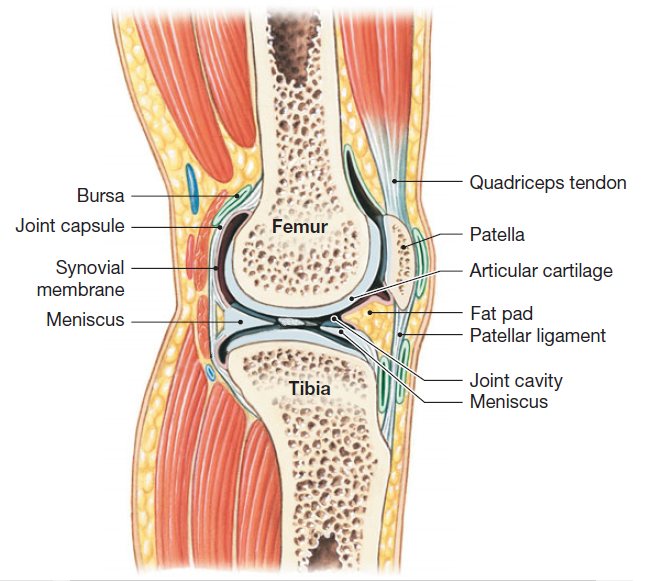
\includegraphics[width=0.7\textwidth]{figures/bonestruc}
\caption{The figure illustrates the anatomy of the knee with focus on the ligaments. Edited from \citep{Martini2012}.}
\label{fig:bonestruc}
\end{figure}

\noindent
It is shown at figure \ref{fig:bonestruc} that the patella is a sesamoid bone, which at birth consists of cartilaginous and ossifies when the child’s extremities gets stronger, which typically proceeds between age two or three and the beginning of the puberty. 
The patella is surrounded by the tendon of the quadriceps femoris. Quadriceps femoris is the muscles which controls the extending of the knee. The quadriceps tendon is combined to the surface anterior and superior of patella. Tibia is combined to the anterior and inferior surface of the patella by the patellar ligament. The bones, tibia and femur, are covered by articular cartilage, which purpose is to protect the bones from friction. The articular cartilage on the two bones are separated from one another by synovial membranes that contains synovial fluid, that further reduce the friction. The primary functions of the synovial fluid is to lubricate, distribution of nutrient and absorption of shock.\citep{Martini2012}

Between the articular cartilage is the fat pads and menisci placed. The fat pads’ function is to protect the cartilage and fill out space as result of the joint cavity changes. The menisci stabilize the knee and acts like pads, that conform shape when femur moves. In addition to fat pads and menisci acts bursa as friction minimization between patella and tissues.\citep{Martini2012} \\
There are three separate articulations in the knee joint, which is one between the patella and the patellar surface of the femur and two between the femoral and tibial condyles. Additionally, the knee consist of seven major ligaments that stabilize the knee joint, which shown as figure \ref{fig:knee}.\citep{Martini2012}

\begin{figure} [H]
\centering
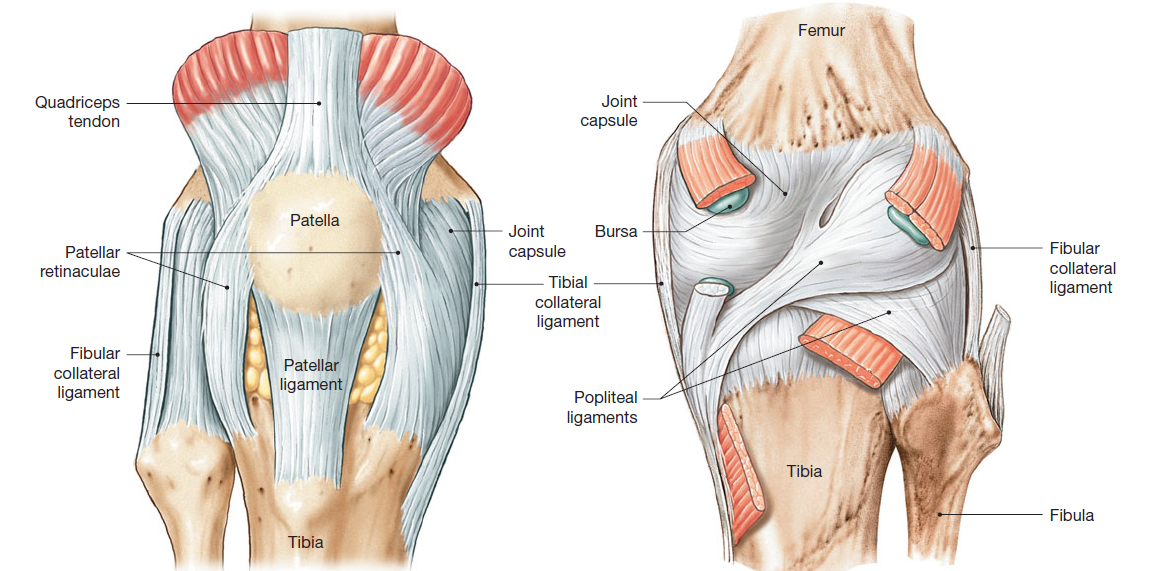
\includegraphics[width=1\textwidth]{figures/knee}
\caption{The figure illustrates the anatomy of the knee with focus on the ligaments. Edited from \citep{Martini2012}.}
\label{fig:knee}
\end{figure}

\noindent
To support the anterior surface of the knee are the ligaments patellar retinaculae and patellar ligament. When the knee is fully extended the tibial and fibular collateral ligament are responsible for stabilizing the joint. Between femur and the two lower bones in the leg, tibia and fibula, is there two popliteal ligaments, which stabilize the posterior surface of the joint. In addition to the visible ligaments in figure \ref{fig:knee} are there anterior cruciate ligament (ACI) and posterior cruciate ligament (PCI) in the joint capsule. The two ligaments cross over each other and are connected to the tibial and femoral condyles. They reduce the movement, anterior and posterior.\citep{Martini2012}

As previously mentioned the gliding joint is formed between the patella and femur, so that during knee movement patella is gliding up and down at the femoral condyle. A condition associated with incorrect movement of the patella, is patellofemoral pain syndrome (PFPS), that occurs when the patella moves outside of its ordinary track, which for instance can be movement in lateral direction.\citep{Martini2012}


\section{Pain}
Pain is experienced and perceived subjectively and there is a lack of methods to measure pain accurately \citep{IASP2012, Younger2009}. 
The International Association for the Study of Pain (IASP) has defined pain as being “an unpleasant sensory and emotional experience associated with actual or potential tissue damage” \citep{IASP2012}.

Physiologically pain can be divided into three categories: Acute pain (less than three months), persistent or chronic pain and cancer pain. Furthermore, pain can be either nociceptive or neuropathic. Nociceptive pain is associated with tissue damage. Neuropathic is associated with damage to the nervous system.\citep{Briggs2010} 

\subsection{Pain mapping}
Pain mapping is a technique, that Harold Palmer introduced in 1949 \citep{Grunnesjo2006}, which is used to transfer a patient’s perceived pain into an objective graph or map by drawing the pain area. Pain drawings can be made by the patients who draw their pain areas on a display on which a body outline is shown, or it can be made by observers who observe the patients and then draw from the signs the patients are showing. An example of a body outline is shown at figure \ref{painmap}. Pain maps can consist of only the drawings, but sometimes a questionnaire is added to get a more detailed overview of the pain.\citep{Schott2010}

\begin{figure} [H]
\centering
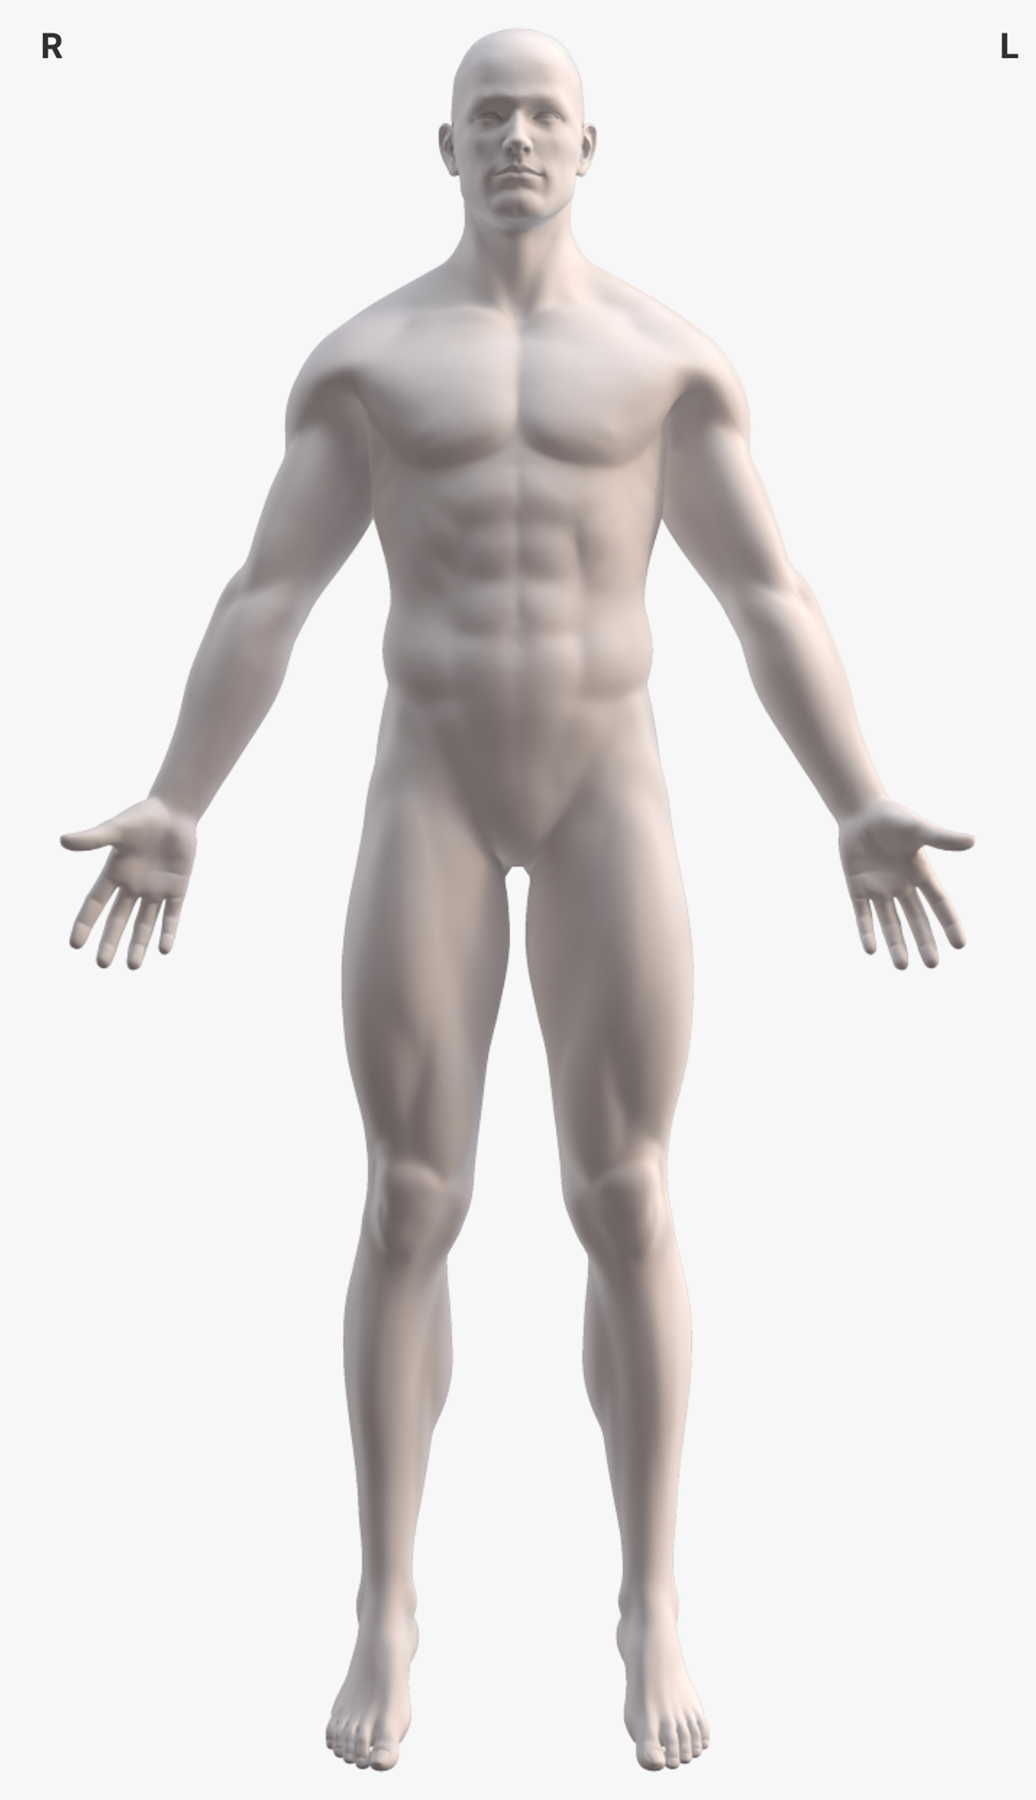
\includegraphics[width=0.4\textwidth]{figures/painmap}
\caption{The figure illustrates a body outline for pain drawing.}
\label{fig:painmap}
\end{figure}

Pain mapping are commonly used in clinical practice \citep{Schott2010}, and can be useful for patients when they try to communicate their pain. Pain maps may also be helpful in diagnosing patients and follow-ups during or after treatment to get an indicator of the patient’s response to the treatment.\citep{Boudreau2016}
According to \citeauthor{Schott2010} there are some issues with the graphical representations of pain, some of which are problems with drawing a three-dimensional feeling of pain on a two-dimensional surface, and distinguishing between internal and external perceived pain on a map.\citep{Schott2010}

\subsubsection{Knee pain regions}
Patients with PFP often describe the knee pain as a diffuse pain, and when looking at pain drawing samples from multiple patients it is also evident that there is a high variability in how pain patterns are distributed across different areas of the knee. 
To distinguish between different pain areas, the knee can be divided into various regions as seen in \autoref{fig:atlas}, where atlases of the left and right anterior knee are illustrated. The atlases has been provided by Shellie Boudreau. 

\begin{figure} [H]
\centering
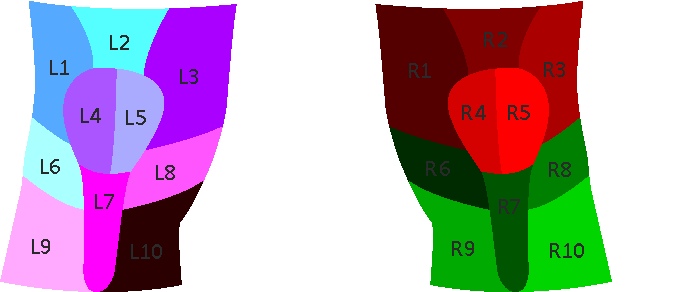
\includegraphics[width=0.6\textwidth]{figures/atlas}
\caption{The figure illustrates atlases of the left and right knee.}
\label{fig:atlas}
\end{figure}

\newpage
\section{Machine learning}
Machine learning describes the use of algorithms to make a system able to identify different data types, like images or text, for transcription of speech into text, matching news items, posts or selection of relevant results of search \citep{LeCun2015}.
Machine learning is a method that uses inductive inference in order to identify rules in a dataset from given input and output \citep{Nielsen2010}. If the computer learns this feature, it can be used to make intelligent decisions and predict specific outcomes.\citep{Nielsen2010}
It is a field that has seen a lot of progress over the past decades, partially because developers recognize the ease in training a system only using examples of the desired in- and output behavior. This is simply easier than trying to manually write a piece of code that anticipate different scenarios from different input types.\citep{Jordan2015}



\subsection{Deep Learning}
Deep learning is a branch of machine learning. The main difference between the use of machine learning and deep learning, is that machine learning is not suitable for handling raw data form. Instead a machine learning system often needs a feature extractor, that will generate a feature vector from the data that can be used as an input for the machine learning system.
Deep learning is based on different techniques that makes it able to handle that data in its raw form, mainly because of its structure.\citep{LeCun2015, Schmidhuber2015} Because of this the system will automatically detect the necessary representations needed for classification and detection. Neural network is a structure of deep learning which consists of different layers, that can be divided into a input-layer and an output-layer, with one or more hidden layers in between \citep{Schmidhuber2015}. The key aspect of these layers is that the features are not defined by programmers, but they are found and learned from raw data using a general–purpose learning procedure.\citep{LeCun2015} An example of the structure can be seen in figure \ref{fig:NN_structure}.   


\begin{figure} [H]
\centering
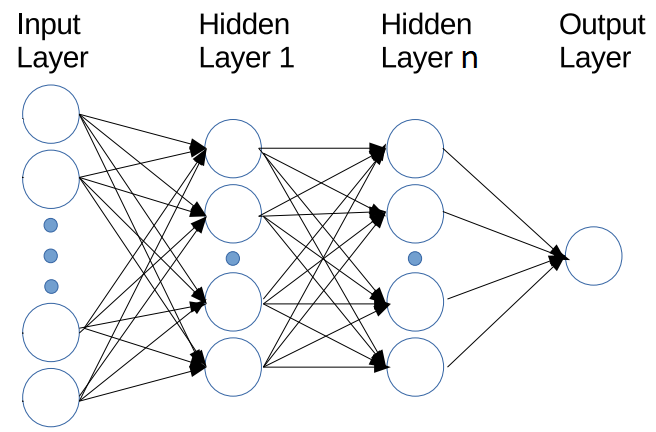
\includegraphics[width=0.6\textwidth]{figures/NN_structure}
\caption{Example of the neural network with possible layers\citep{Acquarelli2017}.}
\label{fig:NN_structure}  
\end{figure}

\noindent
The different layers consist of a series of nodes, where each node is connected by weights to one or several other nodes from a different layer. In the input-layer the nodes are fed with the data that the system is given. The second layer will then receive the output from the previous layer, and this process continues through the layers until the output-layer is reached.\citep{Schmidhuber2015} An example of how the hidden layers affect an image can be explained as follows:  
Firstly, the system detects minor changes like edges. Secondly, the edges are compared and put together to make up different kind of shapes. In the third hidden layer, it will be further combined to make up an object that can be identified.\citep{LeCun2015}

\subsubsection{Learning scenarios}
There are three main learning scenarios: supervised, unsupervised and semi-supervised learnings.

Supervised learning is the most common way of training in machine learning \citep{LeCun2015}. When using this method the system is trained with labeled data, where the generated output can be compared with an expected output, and thereby see how accurate the system is. The weights are interconnection between two layers and they work as a set of coefficients, defining an image feature.\citep{Hameed2016} By adjusting weights inside the neural network it is possible to fit the model better to the training data, and thereby increase its accuracy and reduce error \citep{LeCun2015}. Supervised learning is mostly associated with classification, regression, and ranking problems \citep{Mehryar2012}.

Differently from supervised learning the input in unsupervised learning is received with unlabeled data and the predictions. Then the system organizes the data by searching for common characteristics \citep{Mehryar2012}. An example of an unsupervised learning algorithm is clustering, where the unlabeled dataset goes through a classification, and split into different classes.\citep{Goodfellow2016} 

In semi-supervised learning the learner is receiving both labeled, unlabeled data and then it search for common characteristics in data. It is used mainly when the labeled data is hardly collected and unlabeled data is easily reachable.\citep{Mehryar2012}

\subsection{Convolutional Neural Networks}
Convolutional neural networks (CNNs) perform highly in several tasks, including digit recognition, image classification and face recognition. The key aspect of CNNs is to automatically learn a complex model by extracting visual features from the pixel-level content.
CNNs are feed–forward models that map input data with a set of suitable outputs. 
Accuracy and performance rely on large training datasets and training procedure based on back-propagation with optimization algorithm such as gradient descent which is used for finding minimum value of the function.\citep{Acquarelli2017}

\subsubsection{Back-propagation}
Back–propagation is a popular learning algorithm in CNN. It is valuable because of the simplicity and computationally efficient \citep{Bengio2012}.
The basic idea behind it is to minimize the overall output error as much as possible during the learning stage. This algorithm process is divided in two main stages: forward and backward. In the first process (forward), the back-propagation architecture is described as  the inputs and weights multiplication of each node (separate input) summed with  additional coefficient called biases.\citep{Hameed2016} 

\begin{comment}
It is defined by:
%H(j)=b_in+∑_(i=1)^N▒〖x_i w_ij 〗
Where: x – the inputs, i – neurons, w_ij – weights, j – neurons for hidden layer, b_in – biases
\end{comment}

In the backward process, weights will be updated to minimize the error between input and output layers.
This process will be applied until optimal weights with minimum error is reached.\citep{Hameed2016}




%----------------------Methodology---------------------------
\chapter{Methodology}
*** OPS! IKKE RIGTIGT! ***
This chapter creates an understanding of the given data and the different programs respectvely the program where pain maps are created and the program for development of the neural networks. 

\section{Data}
*** OPS BIRGITHE AND LINETTE REWRITE! ***
Data used in this project were collected beforehand from an on-going FOXH trial which is conducted in collaboration with Danish and Australian universities. The data consists of pain maps which were drawn by subjects with PFP through the use of an application Navigate Pain in a clinical setting. The data contained information regarding the subjects in terms of i.a. age, gender, height and weight. For each individual subject information related to the PFPS was also collected, regarding the duration of PFP, pain intensity and which knee was the most prominent for pain. 
The number of samples available during this study was collected from 217 subjects with PFP. An example of a pain drawing can be seen in figure \ref{fig:kneepainmap}. 

\begin{figure} [H]
\centering
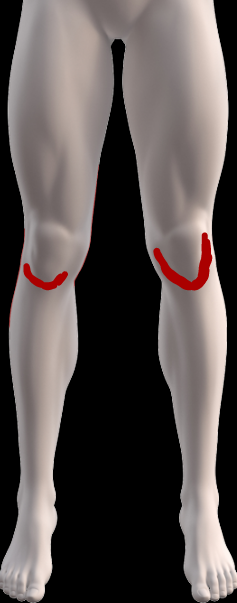
\includegraphics[width=0.25\textwidth]{figures/kneepainmap}
\caption{Pain drawings of the lower extremities. The red markings indicate the area of pain perceived by the individual subject. In this case the PFP is bilateral (on both knees).}
\label{fig:kneepainmap}
\end{figure}

\subsection{Software application: Navigate Pain}
Navigate Pain is a software application that is used to visualise the location, shape and spatial distribution of pain from patient to healthcare personnel. The application permits individuals to draw their pain into a body outline with different colors and line thickness. Navigate Pain android was developed at Aalborg University and a commercial web application is available at Aglance Solutions (Denmark).\citep{Solutions2015}
\autoref{fig:Navigatepain} illustrate the process using the application.

\begin{figure} [H]
\centering
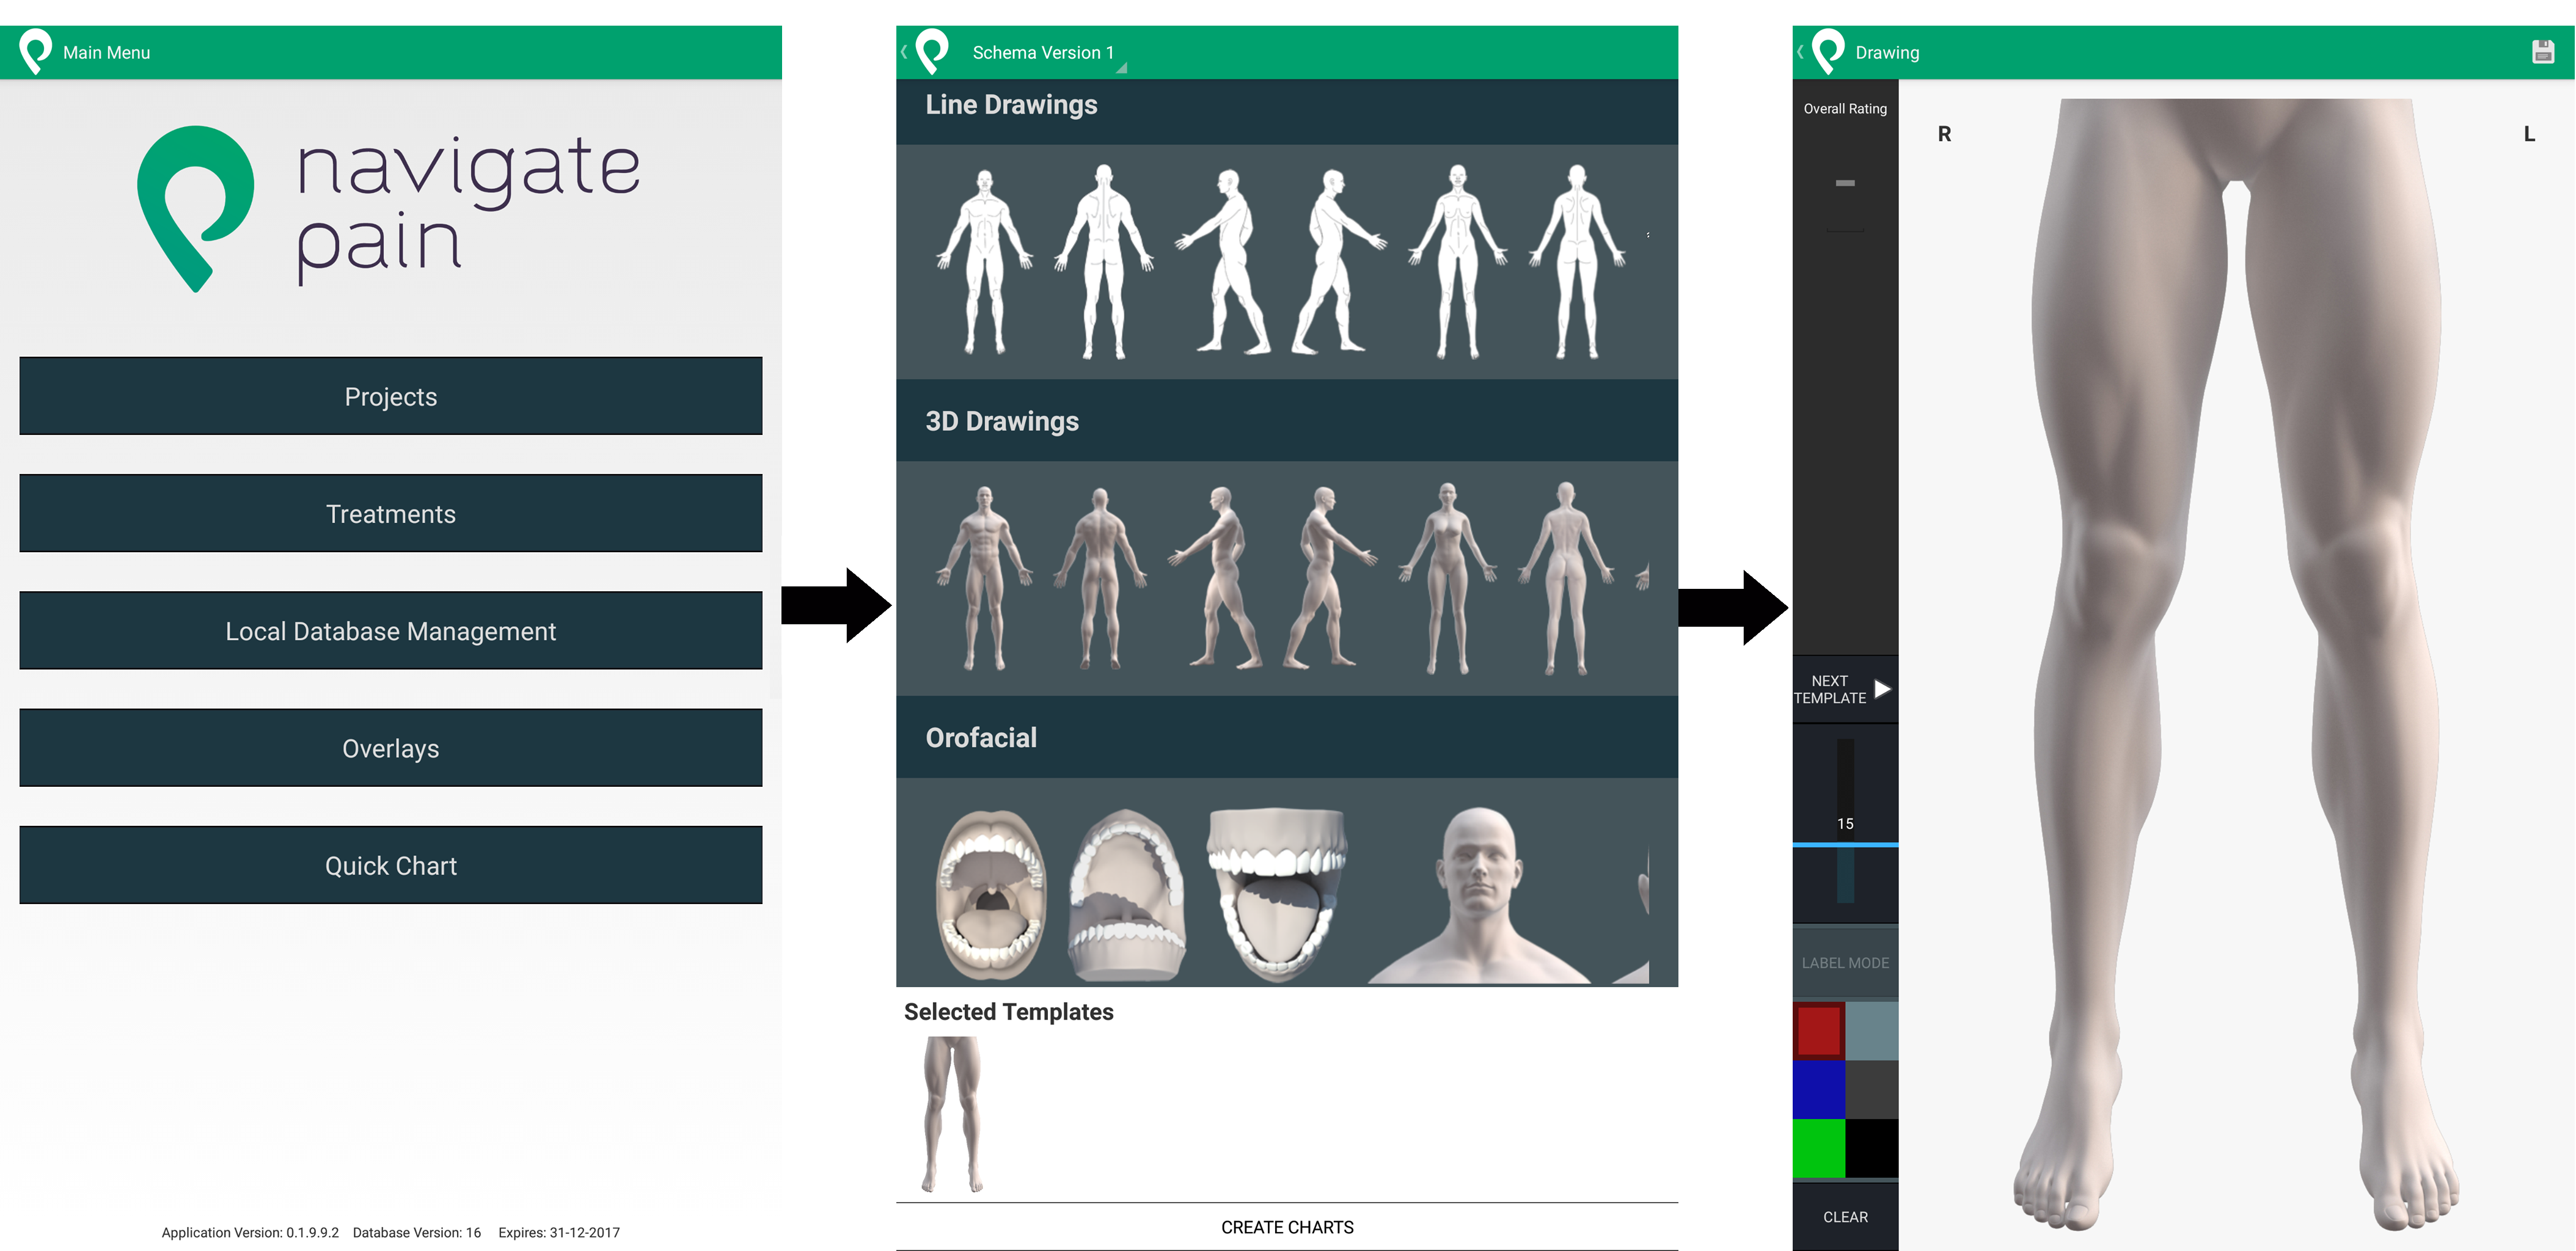
\includegraphics[width=1\textwidth]{figures/Navigatepain}
\caption{The figure illustrates the process for making a pain map with Navigate Pain. There is three screenshots of the application.}
\label{fig:Navigatepain}
\end{figure}

\noindent
The left screen in figure \ref{fig:Navigatepain} is the main screen. By clicking on "Project" a folder with subjects is created. From each subject information like name, age, height is saved. Before the subject can draw their pain areas, the body outline has to be chosen, which illustrates the screen in the middle. The body outlines is divided into five categories: Line Drawings, 3D Drawings, Orofacial, Special Zooms and Knee Pain. In the bottom the seleceted templates is shown. When clicking on "CREATE CHARTS" the right screen is shown. Here it is possible to draw the pain areas with different colors and line thickness, which can be seen in the left side of the screen. Afterwards the pain map can be saved. 

\subsection{Data handling}
BIRGITHE AND LINETTE



\subsection{Data representations}
It is presumed that different data representations of pain maps affect the performance
accuracy of a deep learning model, which is why different data representations are created. 
A study found a correlation between a prolonged symptom duration and the size of the pain area. It was shown that the pain area increased for individuals that have a symptom duration for more than five years compared to those with a symptom duration below five years. Likewise pain intensity had a correlation with the size of pain area for symptom duration above five years. Furthermore, the shape of the pain developed from a U-shape to an O-shape for individuals with a symptom duration above five years.\citep{Boudreau2017} Based on this study the morphology is considered to be relevant to investigate, which is why morphology is one of the data representations.\\

\noindent
The PFP is often described as diffuse pain and therefore difficult to describe and localise \citep{Witvrouw2014}. To accommodate this is it chosen to divide the pain into different knee regions, which may indicate whether a specific region of the knee influence the PFP. This is converted to a simplified data representation that indicate active knee regions. 
A combination of the two data representation is combined to create a third data representation which both include the morphology of the pain and the different knee regions. 
Gender is included as an input parameter in the three data representations, because it is shown that the prevalence is more than twice as high for females than males \citep{Petersen2013, Rathleff2015}.  

\noindent
Since the symptom duration of PFP seems to affect the size and shape of the pain area, is it chosen to classify the three data representations in proportion to symptom duration. Likewise is it chosen to classify pain intensity because of the influence from the size of pain area.
The three data representations is referred to as morphology-representation, regions-representation and superimposed-representation.


\section{Pre-analysis}
The pain maps and associated symptom duration and pain intensity are analysed to get an overview of the data. The data is analysed in MatLab, where the distribution of the outputs, symptom duration and pain intensity, are investigated whereafter the classifications to the neural network models are decided. Furthermore the distribution of gender is compared to the literature which states that the prevalence is higher for females than males.
To select the threshold for data representation according to the active pain regions are the pain areas in different pain maps analysed. 
Simple linear regressions of pain area and either symptom duration or pain intensity are made to get a reference to the neural network models. 

\subsection{Classification of data}
The neural networks models have to classify the data representations into categories. To find these are histograms of the outputs created. \\

\noindent
A histogram of the symptom duration associated with the pain maps is illustrated in figure \ref{fig:histoduration}.

\begin{figure} [H]
\centering
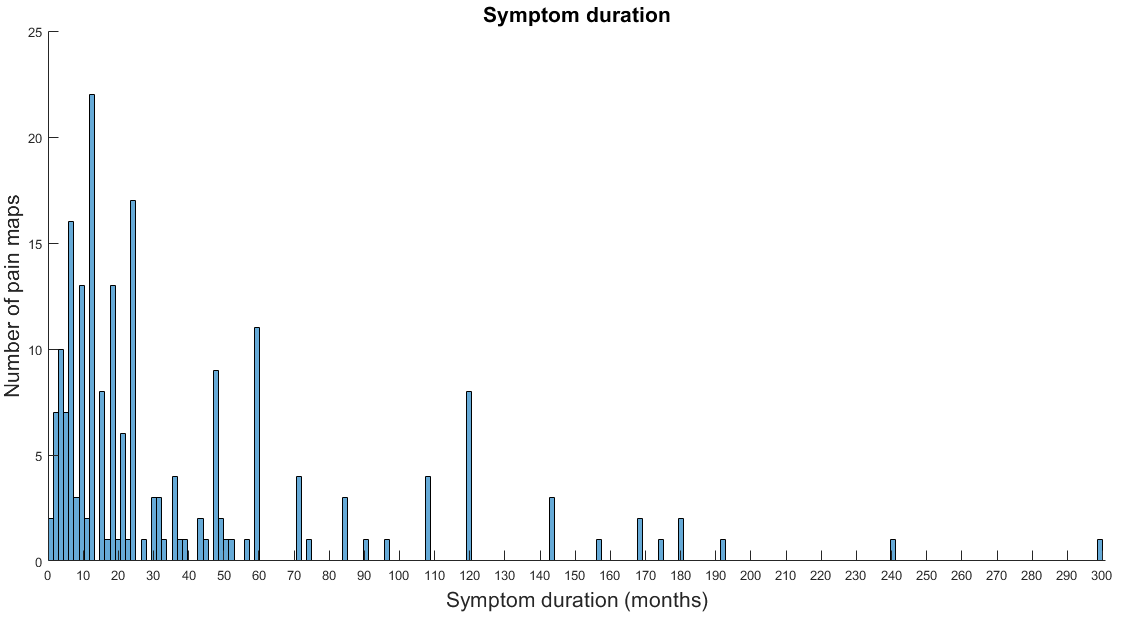
\includegraphics[width=1\textwidth]{figures/histogramDuration}
\caption{A histogram of the symptom duration.}
\label{fig:histoduration}
\end{figure}

\noindent
SOMETHING
hvor mange klasser
hvor de skal splittes 


In the appurtenant data to the pain map the individuals have stated their pain intensity like the worst pain in the last 24 hours and the last 7 days. 
It is not assumably that the individuals have performed any PFP provoked activity in the last 24 hours before drawing their pain, therefore it is chosen to use the worst pain intensity in the last 7 days to get a more average worst pain intensity. 
To explore the difference between the individuals’ stated pain intensity in the last 7 days is a histogram created which can be seen in figure \ref{fig:histopain}.

\begin{figure} [H]
\centering
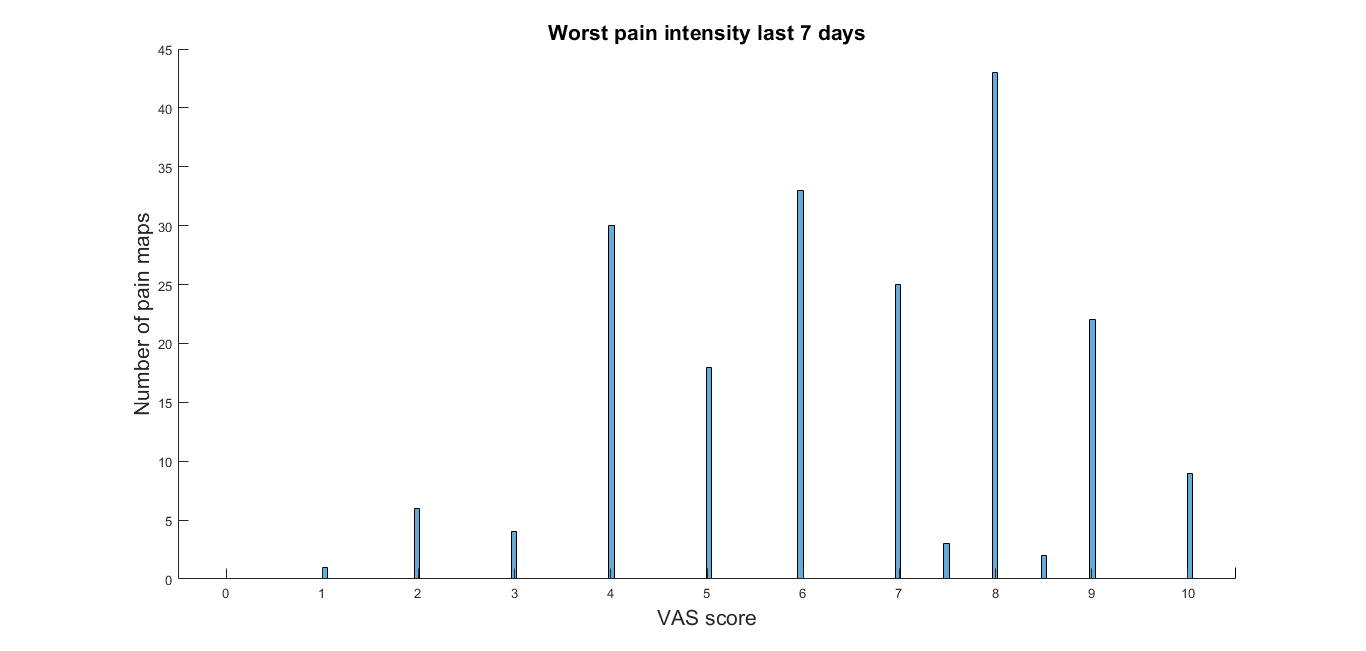
\includegraphics[width=1\textwidth]{figures/histrogramPain}
\caption{Histograms of the pain intensity the last 7 days.}
\label{fig:histopain}
\end{figure}

\noindent
The worst pain intensity is divided into some classes which the models should classify in addition to. To test the models are the data firstly divided into the extremes, since it is assumed that if the models predict badly with the extremes, the models would not predict better with multiple classification of the pain intensity. The extremes is chosen to be intervals 1 to 4 and 8 to 10 by which the last classification constitute the interval between. 


\subsection{Distribution and threshold}
Gender is an interesting parameter to use as an input, because the prevalence is more than twice as high for females than males. Thereto perceived pain is subjective and depends on the individual's character and personality. The distribution of gender is investigated by creating a histogram, which is shown in figure \ref{fig:histogender}. 

\begin{figure} [H]
\centering
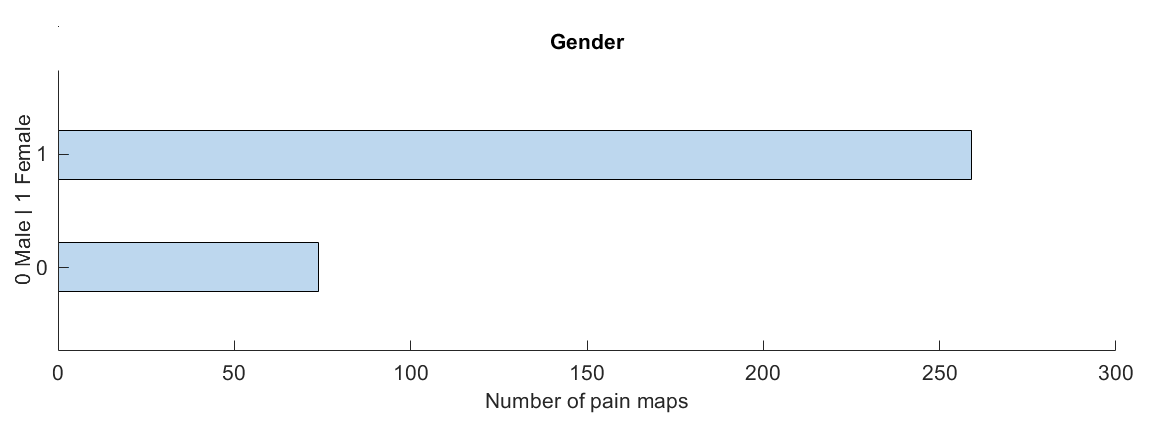
\includegraphics[width=0.5\textwidth]{figures/histoGender}
\caption{Histograms of the distribution/division of gender.}
\label{fig:histogender}
\end{figure}

\noindent
According to the given data the prevalence is higher for females than males. The females constitute 156 of the 206 individuals.

\noindent 
In relation to the data representation that contains information about the active pain regions, it is necessary to find a threshold that decides when a knee region contains enough pain pixels to be considered active. A threshold is required to increase the confidence of an active pain region by avoiding minimal contributions e.g. small pain areas in the associated regions. Simultaneous may the threshold not be too large so potential pain regions will not be incorporated. The threshold to indicate active pain regions is decided based on an analysis, where threshold values of 0, 5, 10 and 15 percent are tested. The analysis of the threshold is tested on five random pain maps to get a general impression of the data. To better illustrate the division of the pain regions are the regions in figure \ref{fig:atlas} colored in different colors that are easier to distinguish, which is shown in figure \ref{fig:colorregion}.

\begin{figure} [H]
\centering
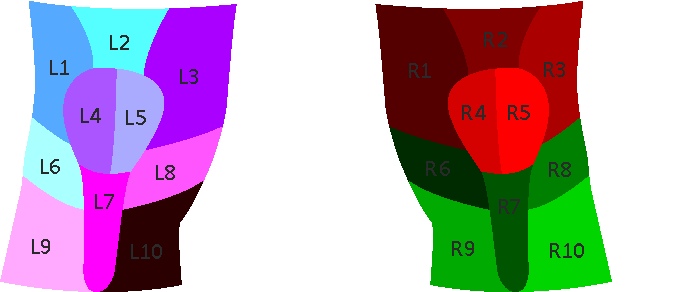
\includegraphics[width=0.7\textwidth]{figures/colorregion}
\caption{Knee regions colored in colors that are easier to distinguish.}
\label{fig:colorregion}
\end{figure}

\noindent
An example of pain maps and appurtenant bar chart are illustrated in figure \ref{fig:threshold}. The pain maps, figure \ref{threshold}(a-d), are likewise colored in the same colors as figure \ref{fig:colorregion} to indicate which regions that are affected according to 0, 5, 10 and 15 percent threshold. The last figure (e) is the bar chart that indicates how many and which active regions there are according to the threshold values.

\begin{figure} [H]
\centering
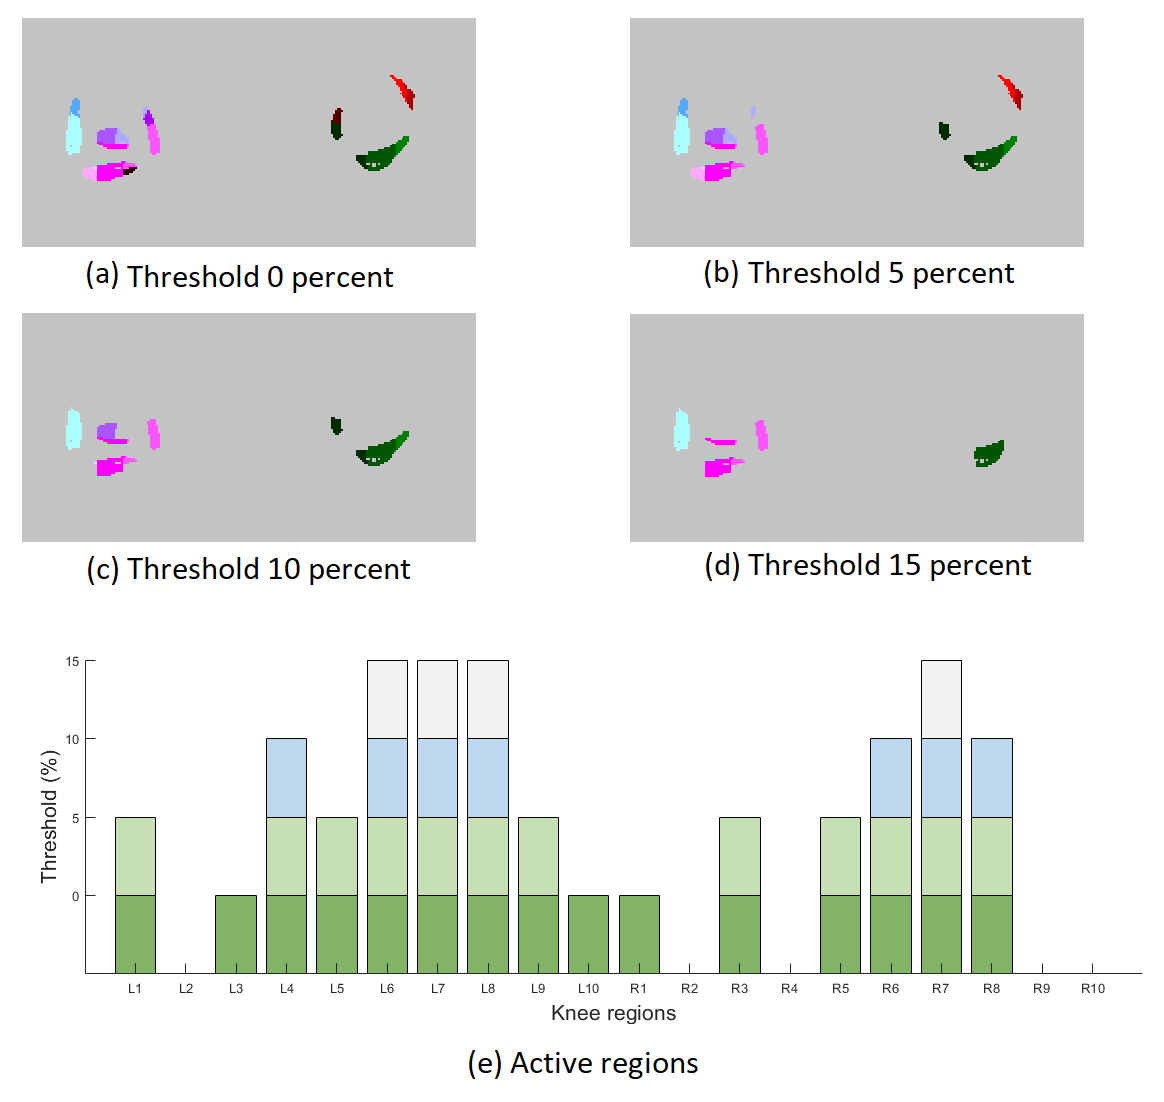
\includegraphics[width=1\textwidth]{figures/threshold4}
\caption{The active knee regions when the threshold is (a) 0 percent, (b) 5 percent, (c) 10 percent and (d) 15 percent. (e) is the bar chart that indicates how many and which knee regions that are considered active.}
\label{fig:threshold}
\end{figure}

\noindent
According to figure \ref{fig:threshold} (a) and (e) is it shown that the knee to the left has nine active regions and the knee to the right has six active knee regions, when the threshold is zero. In proportion to the active regions are region L3, L10 and R1 very small and are thereby the first regions to be discarded when the threshold is increased by five percent, which is shown in figure (b). 
By comparison figure (a) and (b) are there minor changes according to the missing regions, compared to figure (c) and (d) where greater areas disappears after increasing the threshold to 10 and 15 percent. 

Based on analysis of the five pain maps and bar charts, figure \ref{fig:threshold4} and appendix \ref{app:XX}, is a threshold on five percent chosen to avoid including minor pain areas, like L10, as active knee regions, and to avoid discarding too many and large areas, like R3 and R5.


\subsection{Simple regression models}
To test whether there is a linear correlation between the size of the pain area and the symptom duration and pain intensity, are simple regression models made. If the size can predict the symptom duration and pain intensity, it may not be significant to investigate pain morphology and location.

In figure \ref{fig:durationRegression} is a linear regression fit of symptom duration and size of pain area illustrated. 

\begin{figure} [H]
\centering
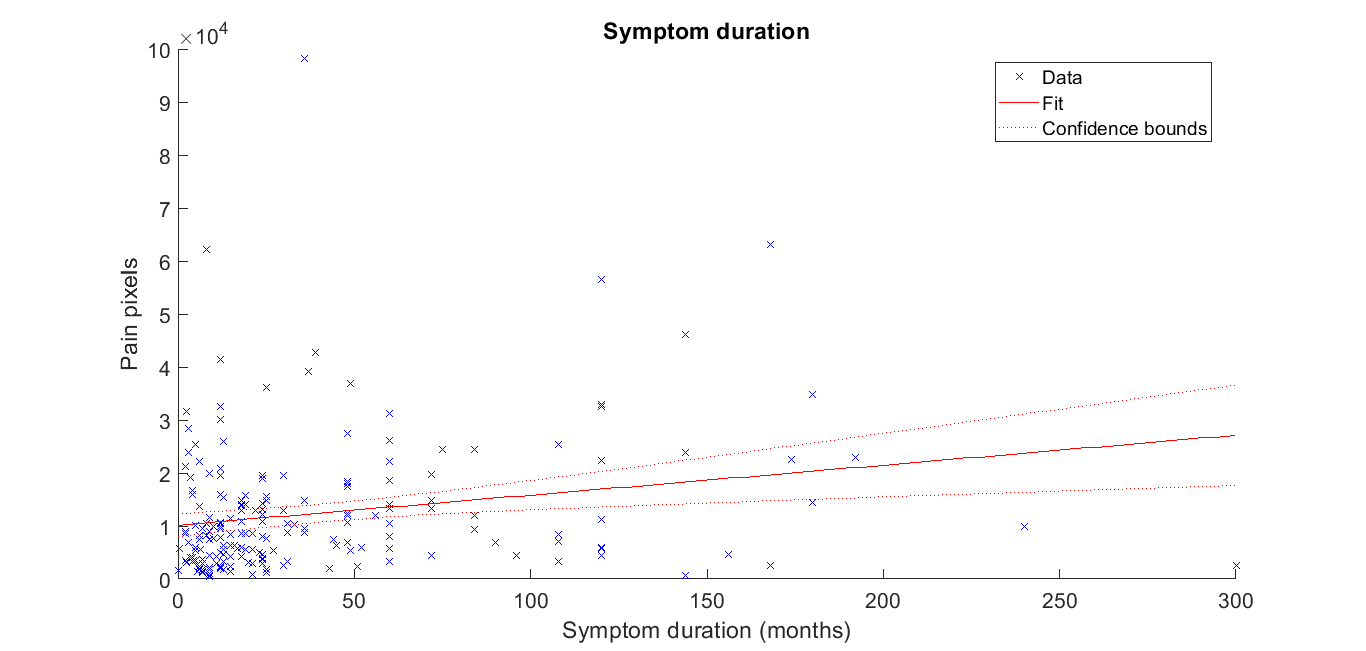
\includegraphics[width=1\textwidth]{figures/durationRegression}
\caption{A simple linear regression fit of symptom duration and the size of pain area.}
\label{fig:durationRegression}
\end{figure}

\noindent
The linear regression model of symptom duration has an R-squared value of 0.046, which is close to zero and therefore the model is not a good fit for the data. 
A linear regression model of pain intensity and the size of pain area is also made, which is illustrated in figure \ref{fig:painRegression}.

\begin{figure} [H]
\centering
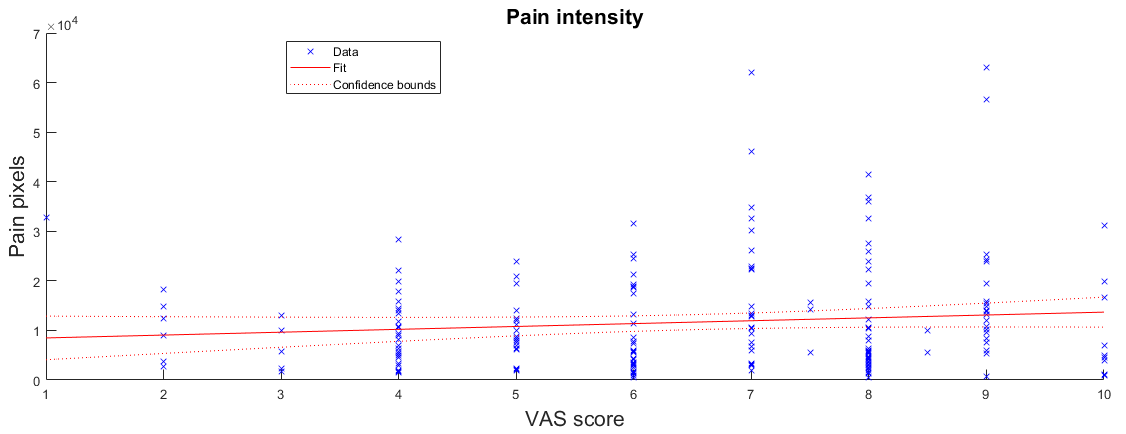
\includegraphics[width=1\textwidth]{figures/painRegression}
\caption{A simple linear regression fit of pain intensity and the size of pain area.}
\label{fig:painRegression}
\end{figure}

\noindent
The R-squared value of this model is 0.0117, so the linear model is not a good fit on the data. 
These linear regression models are not very suitable when trying to predict symptom duration or pain intensity from the size of pain area. However they can be compared to the performance of the neural network models.  



\section{Pre-processing}
The data is pre-processed in MatLab to prepare it to the three different neural network models. Each model has an appurtenant data representation which are prepared in three different ways. The three data representations are morphology, regions and superimposed morphology and region. Common for the data representation is that the pain maps are imported as image-matrices whereafter the matrices are resized, since the given data was collected at different resolutions (screen sizes). Furthermore, the matrices are cropped to sort out unnecessary data like the areas inferior and superior to the knee.
Before the data is used as an input in the neural network models, the image-matrices are converted into vectors whereafter they are assembled in one matrix for each data representation. To get additional information associated with the pain maps, is gender added by including a column vector to the three matrices. 
In addition to the input, the neural network models need an output to train the models. The output, which is either symptom duration or pain intensity, is likewise added as a column vector. 
The following sections describe the pre-processing of the individual data representations. 

\subsection{Morphology-representation} \label{sec:Morph}
The first representation of data is a binary matrix of the original pain maps.
Firstly, the image of the original pain map is gray-scaled to get a one-dimensional matrix instead of a three-dimensional RGB-matrix. This matrix is then converted into a matrix consisting of zeroes and ones, where the pain pixels are symbolized with ones. An original pain map and a pain map consisting of a binary matrix is shown in figure \ref{fig:cropbin7}.

\begin{figure} [H]
\centering
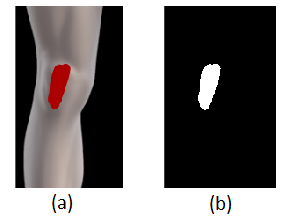
\includegraphics[width=0.7\textwidth]{figures/cropbin7}
\caption{(a) Original pain map and (b) image consisting of a binary matrix where white color represents the pain pixels.}
\label{fig:cropbin7}
\end{figure}

\noindent
An illustration of this data representation is created to convey how the data is assembled and transferred to the model. The illustration is shown in figure \ref{fig:binmatrix}.

\begin{figure} [H]
\centering
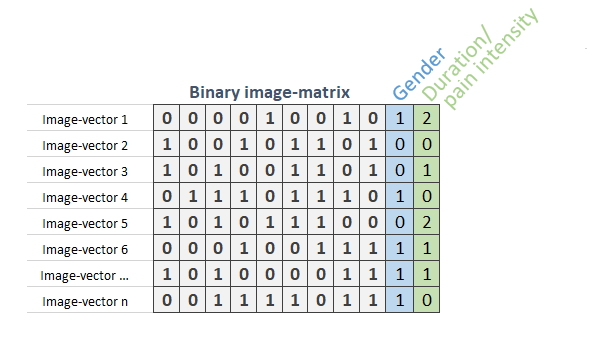
\includegraphics[width=0.8\textwidth]{figures/binaryimagematrix}
\caption{An illustration of the matrix of the morphology data representation. The matrix consist of image-vectors for each subjects where the two last column indicate the appurtenant gender and either duration or pain intensity. The image-vectors has a length equal to the number of pixel in the pain maps.}
\label{fig:binmatrix}
\end{figure}


\subsection{Regions-representation}
The second representation of the data is a matrix consisting of vectors with 20 values which indicate pain in relation to the knee regions.
The knee regions shown in figure \ref{fig:atlas} are converted into a matrix consisting of 20 values, which represent each knee regions. This matrix is superimposed to the binary image of the pain map, which results in a matrix with pain represented in each knee region. In figure \ref{fig:binregions} are the knee regions and the pain associated with the regions illustrated.

\begin{figure} [H]
\centering
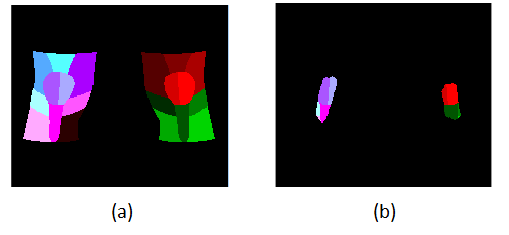
\includegraphics[width=0.8\textwidth]{figures/binregions}
\caption{(a) Knee regions and (b) pain in the specific regions.}
\label{fig:binregions}
\end{figure}

\noindent
After superimposing the two matrices, knee regions and pain, the number of pixels in each active knee region is found. This number is compared to the total number of pixels that are in each knee region, so knee regions with less than 15 \% pain are excluded. WHY 15\%. As a result a vector with 20 values is created. This data representation is implemented the same way as the first representation, figure \ref{fig:binmatrix}. The only difference is that the length of the image-vectors respond to the 20 regions, and therefore are there only 20 values in this data representation.


\subsection{Superimposed-representation}
The third representation of the data is a matrix consisting of individuals’ pain divided into the knee regions.
\noindent
In this representation the superimposed matrix from the second data representation is used. Since the data representation should reflect the morphology of the pain and divide the pain into the different knee regions is one-hot encoding used. One-hot encoding is a way to separate categorical data into binary data \citep{Harris2012}. This means that the 20 values for each knee region do not have a correlation. After one-hot encoding the superimposed matrix consists of 20 layers where each layer represents a knee region. An illustration of this data representation is shown in figure \ref{fig:onehot}.


\begin{figure} [H]
\centering
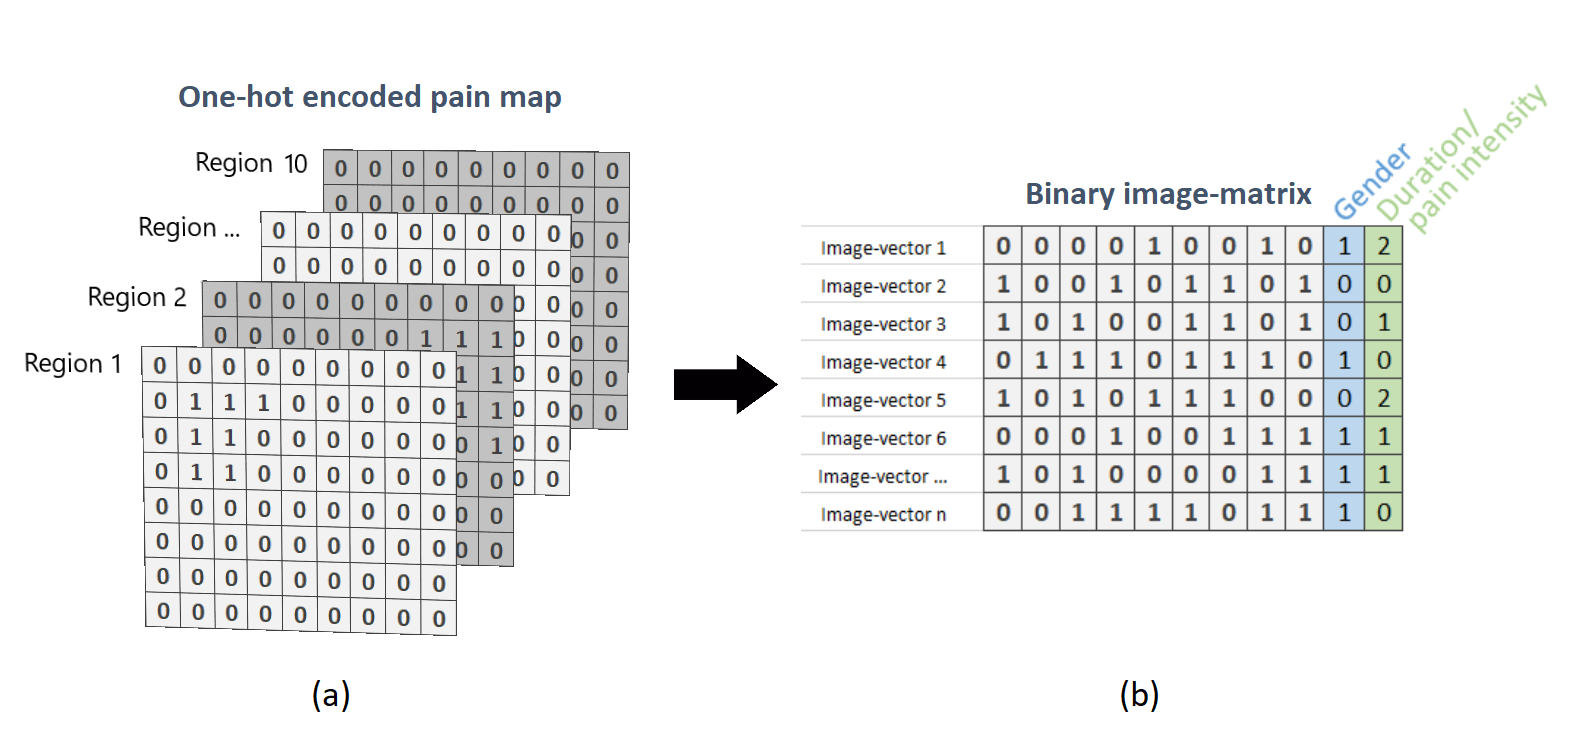
\includegraphics[width=1\textwidth]{figures/onehotmatrix}
\caption{(a) illstrates the one-hot encoded pain map and (b) shows the images-vectors in one assembled matrix with gender and either symptom duration or pain intensity.}
\label{fig:onehot}
\end{figure}



\section{Neural network implementation and models}
Building neural network for classifying pain maps was try and error process.
In this project the deep learning method is used to classify the pain maps and gender by determined outputs. The data is a set of 2D-images combined with gender and the outputs are pain intensity and duration. For classification purpose supervised convolutional neural network is used followed by fully-connected layers at the end. This architecture of the model is chosen to the interest of morphology and location of the pain. as there was no "golden recipe" for most optimized  The models are trained and tested on a single computer with GPU and ran on Python programming language with Keras library and Tensorboard tool for visualizing results. Specifications of hardware and software are described in detail in section {Sofware and hardware}.

\subsection{Sofware and hardware}
In this project it is chosen to use Python v3.6.3 for development of the neural network. Python is an object-oriented and general-purpose programming and scripting language. Python is among other things used for programming websites, mobile applications, desktop GUI's, but also used for machine learning programming.
When developing a machine learning application, there are different libraries that can be used, where some of the most popular is the Theano and the TensorFlow and Keras libraries.\citep{Swamynathan2017}
The model was created and tested using Keras library, which is a high-level neural networks API (Application programming interface). Keras runs on top of either TensorFlow or Theano. Keras is a simplified version of the two libraries, which makes it easier to program in Python, but still allows for building complex models. TensorFlow is an open source library for development of machine learning applications, that has been released by Google \citep{Swamynathan2017}. 
Using CPU or GPU on this platform the most mathematical operation  is computed in a computerized and simple way \citep{Swamynathan2017}. A small example of the concept of using TensorFlow could be seen in Appendix B. The plots for this model are generated using Tensorboard visualizing tool. It allows to watch a graph during the training, gives plot quantitative metrics and shows data like images that pass through it. Besides visualizing part of this tool it is also useful for debugging as it allows to observe the graph at a present time.\citep{Abadi2016a}

\noindent
The classifier was created on a machine with 4x ‘‘Intel® Core™ i7‘‘ CPU‘s and one single GPU of type "Geforce GTX 970M" with specifications listed in table \ref{fig:Specs}.

\begin{figure} [H]
\centering
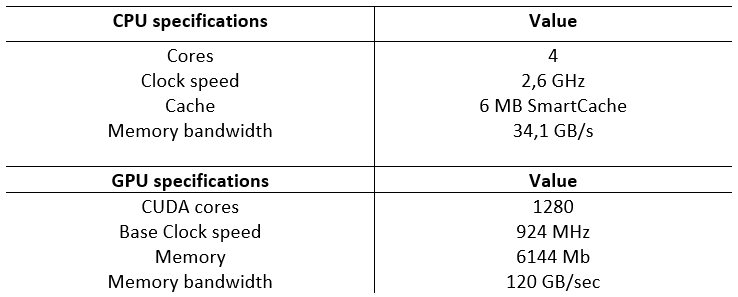
\includegraphics[width=1\textwidth]{figures/Specs}
\caption{Specifications of CPU‘s and GPU \citep{Intel,Nvidia}.}
\label{fig:Specs}
\end{figure}

\subsection{Data handling and design choices of the models}
This section presents the different models used, their architecture and implementation.
The models will be operating on a pixel level by learning features of the pain charts.
Each model will be using fully connected layer concept discussed in \autoref{sec:Layers}, and equal optimization methods. Convolutional layers will be used only on morphology and combined representations of data, while region representation containing labelled knee areas runs on fully connected layers.
Instead of including all pain maps from the dataset, validation and test set were specified separately. 10-fold cross validation technique were used calculate the average accuracy, specificity and sensitivity. Each model will be used twice to independently test the generalization performance of pain duration and intensity. Supervised learning is used for training in all the models. The generic input for all of the model is gender, along with the different image representation, which are presented in figure \ref{fig:Schema1}. These inputs are trained and then compared against their respective category label. 

\begin{figure} [H]
\centering
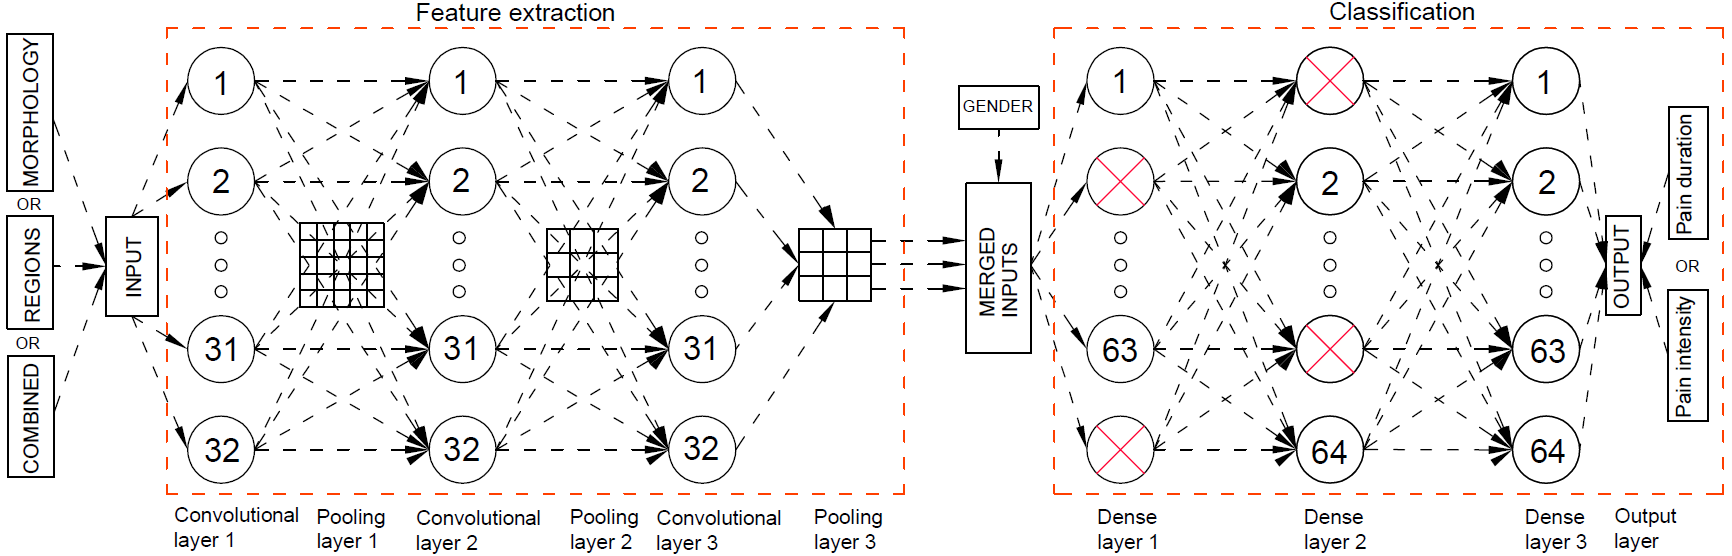
\includegraphics[width=1.0\textwidth]{figures/Schema1}
\caption{Architecture of the neural network model used for this study.}
\label{fig:Schema1} 
\end{figure}

From the higher point of view, the model can be architecturally split into two main parts. Feature extraction part, where convolutional and pooling layers alternates in order to extract the most important features out of the image. Second part is called classification, where computed feature maps will be assigned to particular class of the output layer. In order to obtain a higher generalization performance of deep learning classifier, methods like activation function, regulation and optimization will be used within the layers were implemented into the models.

\subsubsection{Morphology - representation model}
The pain map representation of morphology works as input of the model, where the input layer is a convolution layer. This layer is set-up to receive a input shape of the dimension of the pain map, that is defined during re-scaling of the pain maps in \ref{sec:Morph}. Gender works as secondary input in the second section of the model, along with the pain maps features extracted through the convolution layers. Before the pain maps features reach the fully connected layers it is flattened from a matrix to a single row in order to merge the features with gender. The merged data passes through fully connected layers and reaches the output layer where it is given a percentage value according to which class it fits the most. Morphology model architecture is shown in figure \ref{fig:Schema1}.

\subsection{Regions-representation model}
The architecture for this model only contains fully connected layer, since the data representation only contains 21 element vector that reflects the active pain regions and gender as described in \ref{sec:Regions}. It is evaluated that there would not be any gains in making the model more complex e.g. adding of convolution, based on the information available from vector, since the level of detail in relation to morphology is very simple. The architecture of the model is illustrated in \ref{fig:Simpleschema}.

\begin{figure} [H]
\centering
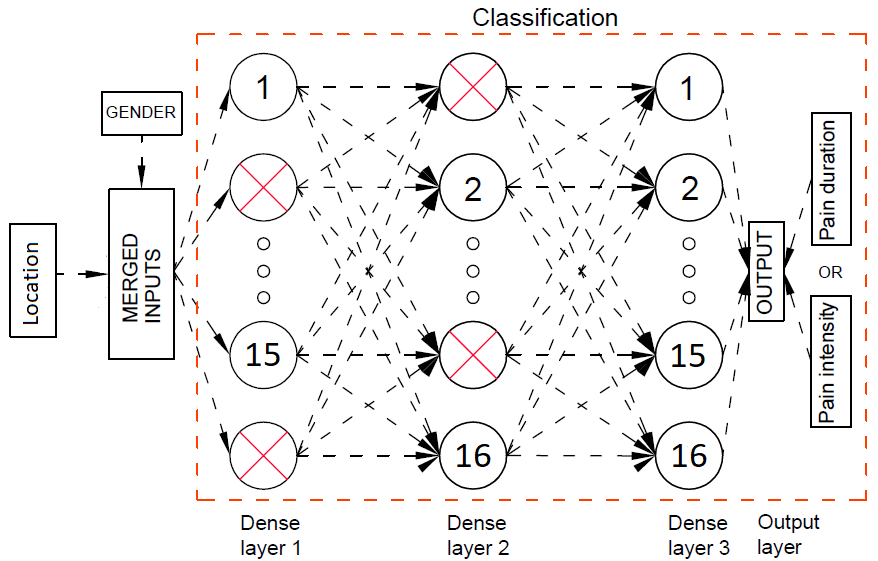
\includegraphics[width=0.6\textwidth]{figures/Simpleschema}
\caption{Architecture of the regions-representation model.}
\label{fig:Simpleschema} 
\end{figure}

\subsection{Combined representation model}
The architecture of this model is nearly identical to that of the morphology representation model.
The main difference can only be seen in the input layer for the pain map representation, where the input shape is altered to contain 20 layers per pain chart instead of one. This is the result of the one-hot encoding done to the images as described in \ref{sec:combined}. 

\subsection{Data handling in python}
The pre-processed data is loaded from a %\textip{.mat} 
.mat file into python.
Data within the file is pre-shuffled and split into a training and test sets, as described in \autoref{sec:pre-process}. The reason for shuffle the data is to improve generalisation through randomization.
In Python the training subset is further divided into a training and validation subsets. 
The training subset is used to find the optimal weights with the backpropagation algorithm \citep{Bengio2012}. In this project, training subset is considered to use up to 75\% of the data. The validation set makes up 15\% of the available data.
The test set will be used to evaluate the generalization of the model, and therefore will not contain data that has been used during the training. By keeping the test set separate it will act as new unseen data, for the model. It contains 10\% of the data.
For the morphology, and combined pain map representations, the images were reshaped from a row vector, back into a matrix to retain their 2D structure.
Furthermore the classification labels were one-hot encoded, so they were compatible to the number of outputs in the models. This is a result of the loss function \textit{categorical\_crossentropy} used for the models, that tries to reduce loss between the categories.    

\section{Optimization}
To try to reduce overfitting and improve generalization of the neural network different techniques are applied network models. Grid search method was used to find most optimal hyperparameters by cross-validating them 5 times and evaluating the mean values with SD. Activation function, dropout, optimizer, learning rate, type of initializer, number of neurons, batch size and number of epochs were tested using this method.  All used optimization techniques are presented in this section and table with used values is presented in FIGURE or RESULTS section (x,x)

\subsubsection{Activation function}
During this study different activation functions, such as ReLu, Softmax, Sigmoid were tested. Results were compared using grid-search and ReLu was picked as activation function for the models. Activation function was implemented in convolutional and fully-connected layers. Sigmoid activator was used for final output layer, because (NEED TO EXPLAIN).

\subsubsection{Dropout}
Dropout is implemented in the models due to the benefits described in section \ref{sec:dropout}. Dropout of three different values were tested on grid-search and 0.5 were picked as it scored the highest. This regulator is only used within the hidden fully-connected layers, where it is defined to randomly drop 50 \% of the nodes. Dropout is shown in figure \ref{fig:Simpleschema} and marked as red crosses. 

\subsubsection{Optimizer}
Adam, RMSprop, Adagrad and SGD, presented in section \ref{sec:optimizers}, were tested and compared. SGD scored the highest and was implemented while compiling the model.

\subsubsection{Learning rate}
In order to determine the most optimal \textit{learning\_rate} for the Adam  and SGD optimizers several different values were tested. Default value 0,001 performed higher than values of 0,01 and 0,0001. To fit the model this parameter was set to 0,001 meaning that the convergence of gradient descent is reached slower but with more accurate \textit{minima}. 

\subsubsection{Batch size and number of epochs}
Three different values of batch size and number of epochs were chosen based on computing power. Grid search on batch size were tested on 5, 10, 15 values, while number of epochs were 15, 25, 35. On every data representations these hyperparameters varied. Batch size and number of epochs were used during the fit process.

\subsubsection{Weight and biases initializing}
Weights and biases initialization was performed, since it affects the performance of the model.
A grid search of weight initializer using \textit{uniform}, \textit{lecun\_uniform}, \textit{normal}, \textit{glorot\_normal} and \textit{glorot\_uniform} were tested and results revealed that \textit{glorot\_normal} performed the best by 3,2 \% compared to the second best. Results can be seen in \ref{pictureFromCMD}. Weight initializer was used in convolutional and fully-connected layers.
Biases were initialized to zeros values
% See image - kernal_init.png 

\subsubsection{Number of neurons}
Number of neurons were chosen based on the best performance comparing 16, 32, and 64 neurons per hidden layer. 32 in convolutionals and 64 neurons in fully-connected layers scored the highest in terms of accuracy. These values were used in in the model within all data representations.

\subsection{Training and validation}
The training was performed using mini-batches of size 10 with SGD optimizer with default learning rate, explained in section \ref{sec:optimizers}. Data was split into train(75\%), validation (15\%), and test (10\%) sets, and the models were regularized using dropout (50\%). Number of neurons in hidden layers were decided to be used as 32 for convolutional and 64 for fully-connected layers. All networks were using ReLu activation function, except output layers, which were using Sigmoid activator instead, described in Section %{activation function}.
The model weight parameters were initialized at random values using \textit{glorot\_normal}, biases parameters were initialized to zero values.

\subsubsection{Stratified m-folds cross-validation}
As a result of binary output, 10-fold cross-validation method were used for training the data and evaluating the performance of the models. Folds were separated 10 times randomly in relation to the distribution of the classes. Stratified m-folding prevents the fold to contain the data of one class. Accuracy, sensitivity and specificity were calculated after each fold and the mean values of these parameters were generated at the end of the training. Results are given in section %{the results}.

\subsubsection{Error and accuracy graphs)}
During each training and validating epoch, the error and accuracy is calculated and presented as graph at the end. According the error graph, the overfitting or underfitting could be determined. Model could be optimized based on these results with technique described in section \ref{sec:optimizers}.

\subsection{Testing}
The testing or prediction refers the generalization performance from the given classification question and is the main job for the neural network.
Separated 10\% dataset were used for testing how accurate the training model can perform using unknown data. By feeding new data into the network, testing process begins. At each time-step classifier predicts the probability for every possible class, and selects with the highest probability as it prediction, giving it as a percentage result. Predictions were presented as a confusion matrix in section {results} providing true positive and negative together with false positive and negative results.


%--------------------------------------------------------------%

%\chapter{Description of models}
%\section{Data handling and design choices of the models}
This chapter presents how the pre-processed data is loaded and prepared for training of the models in Python, as well as the different architectures of the models, and features related to their implementation. Three separate models have been made fitting to each of the data representations described in section \ref{sec:prepros}. 

\subsection{Data handling in python}
The pre-processed data is loaded from a \textit{.mat} file into python.
Data within the file is pre-shuffled and split into a training and test subsets, as described in \autoref{sec:prepros}. 
% The reason for shuffle the data is that improves generalisation through randomization.
In Python the training subset is further divided into a training and validation set. 
The training set is used to find the "optimal" weights with the back-propagation algorithm \citep{Bengio2012}. In this project, training set makes the biggest percentage amount of the data up to 75\%.
The validation set is used for estimating the generalization error of the model, and to examine how adjustments to hyperparameters effect the model performance \citep{Duda2000}. Hyperparameters often define many different values that can be adjusted, to control the behavior of the algorithm, to which some parameters may affect the runtime and computational cost when training the model \citep{Goodfellow2016}.The validation set makes up 10\% of the available data for the different models.
The test subset will only be used to evaluate the generalization of the model, and therefore will not contain data that has been used during the training \citep{Duda2000}.
By keeping the test subset separate it will act as new unseen data, for the model. It contains 15\% of the data.

For the binary, and combined pain map representation, the images were reshaped from a row vector, back into a matrix to retain their 2D structure. 

Furthermore the classification labels were one-hot encoded, so they were compatible to the number of outputs in the models. This is a result of the loss function \textit{categorical\_crossentropy} used for the models, that tries to reduce loss between the categories. This demands that the class label has the same dimension as the number of outputs in the model \citep{Chollet2015}.    

\subsection{Optimization techniques}
To try to reduce overfitting and improve generalization of the neural network different techniques are applied network models.

One method used to automatically chose hyperparameters is used, and is known as grid search \citep{Goodfellow2016}. By using this method a listing of different hyperparameters were tested on a model, that allowed for choosing the parameter that give the highest improvements in performance in relation to the validation loss and accuracy.  

Grid search is mainly practical when there are only a few hyperparameters that needs to be tested, because of the exponentially computational cost follows \citep{Goodfellow2016}.   

\subsubsection{Optimizer used for the models}
The Adam has been implemented in the three models, based on the findings of comparing it to the performance results with stochastic gradient descent optimizer. Adams optimizers showed a higher accuracy and significant higher training speed. Comparison results can be seen in \ref{picture from CMD}
% written in \autoref{deeplearning}.

\subsubsection{Kernel-initializer}
Kernel-initialization was performed, since it affects the performance of the model.
A grid search of kernel-initializer using \textit{uniform}, \textit{lecun\_uniform}, \textit{normal}, \textit{glorot\_normal} and \textit{glorot\_uniform} were tested and results revealed that \textit{glorot\_normal} performed the best by 3,2 \% compared to the second best. Results can be seen in \ref{picture from CMD}
% See image - kernal_init.png 

\subsubsection{Learning rate}
In order to determine the most optimal \textit{learning\_rate} for the adam optimizer a several different values were tested. To fit the model this parameter was set to \textit{0,0001} (lower than default value) meaning that the convergence of gradient descent is reached slower but with more accurate \textit{minima}. It showed the 

\subsubsection{Batch training}
Initial experimentation of the batch size showed little flexibility, because of the available computation power for training of the model. The batch size could not exceed a value of four, by reason of the relative high image resolution (912 x 2315). As a result of this it was chosen reduce the resolution (233 x 251). Resizing of the images, are described in \ref{sec:prepros}.

Furthermore, the grid search of batch parameters were performed with values of 5, 10, 15, 20, and the highest accuracy with the value 5 were chosen

\subsubsection{Cross-validation}
Because the amount of data for this project is limited it is chosen to implement m-fold cross validation, where the training data is divided into \textit{m} number of subsets. Each of the subsets can function a either a validation set or as a part of a training set e.g. if a classifier is trained \textit{m} times, then each time a different subset will be used as a validation set, and the rest is used for training. \citep{Duda2000}
Because of the property of cross validation, it can be used as a way of investigate a general accuracy since all data is included during training, but may not be beneficial for every kind of problem. \citep{Duda2000}

\subsubsection{Dropout}
Dropout is implemented in the models due to the benefits described in section \ref{sec:dropout}. The dropout is only used within the hidden fully-connected layers, where it’s defined to randomly drop 50 \% of the nodes.

\subsubsection{Activation function}
ReLu activation function is used as controlling unit for nodes activation. It defines when the node is considered as active. In the model ReLu is  implemented in convolutional and fully-connected layers.

Sigmoid is implemented only in the output layer, because it 

It has something to with the fact that the output layer performs the classification and needs sigmoid is more sutible for this task then ReLu...   

%Additional info that need to be placed somewhere.% There are simple methods that can be used to improve performance and training speed. Scaling of the input and giving an initial weight \citep{Duda2000}
%Maybe the grid test support this as well, and maybe also something about computation power.and the sigmoid for the output layer. 

\subsection{Training of the networks}
Supervised learning is used for training in all the models. The generic input for all of the model is gender, along with the different image representation, which are presented in /ref{to data}. These inputs trained and then compared against their respective category label.  WE CAN MENTION HERE THE TYPES OF DATA AND TYPES OF MODELS IF THEY ARE NOT PRESENTED LATER

%TEMP CRAP THAT NEEDS TO BE PLACED ELSEWHERE
Temp-placehoder:
The process of making the neural network model has been a trial and error process, because there is not an actual “cookbook” for developing NN (This statement is from a not vaild source, but so far it’s the only one that i have found.) \citep{Goodfellow2016}

\section{Vector image model}\label{sec:SimpleRepModel}
The architecture for this model only contains fully connected layer, since the data representation only contains 21 element vector that reflects the active pain regions and gender as described in \autoref{LinetteAndBirgithe}. It is evaluated that there would not be any gains in making the model more complex e.g. adding of convolution, based on the information available from vector, since the level of detail in relation to morphology is very simple.
The architecture of the model is illustrated in \autoref{fig:simpleModel}.

\begin{figure} [H]
\centering
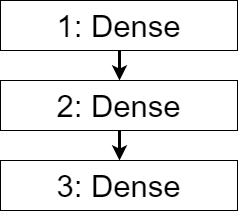
\includegraphics[width=0.3\textwidth]{figures/simpleModel}
\caption{Arcitechture of the neural network using knee region representation.}
\label{fig:simpleModel} 
\end{figure}

The model consists of three layers, where the input and output layer..(WE ADD MORE)

\section{Raw binary representation model}\label{sec:BinaryRepModel}
The architecture of this model is based on the typical structure of a convolutional network, where the first layers alternate between convolutional layers and max pooling layers \citep{LeCun2015}. This defines the first part of the model. The following layers consists of three fully connected layers, and output layer, and defined the second part of the model. An overview of the architecture is shown in \autoref{fig:binaryRepModel}. 
Convolution layer are implemented for this pain map representation, because of their ability to extract morphology features from images, as written in \autoref{CONVOLUTION}

\begin{figure} [H]
\centering
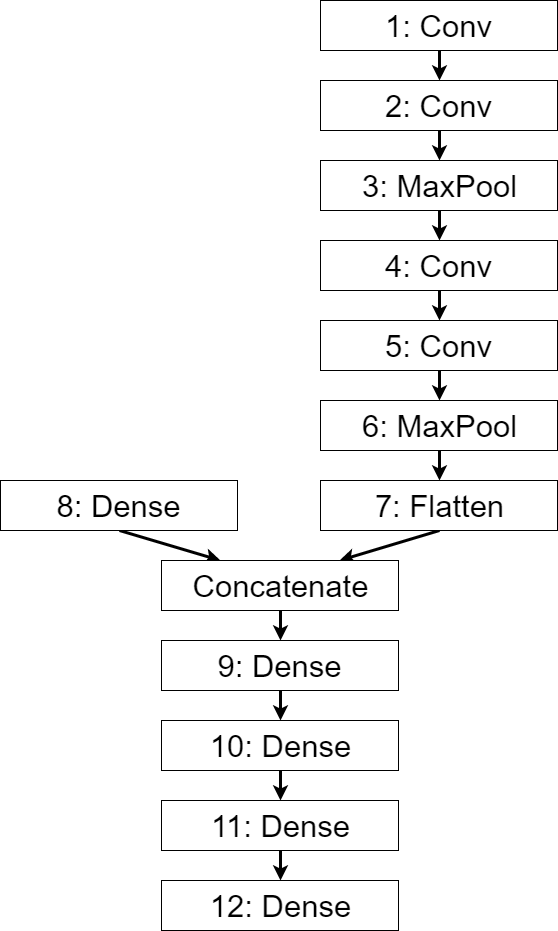
\includegraphics[width=0.6\textwidth]{figures/binaryRepModel}
\caption{Architecture for the neural network model using binary pain map representation. REMEMBER TO INCLUDE THE INPUT IN THE FIGURE}
\label{fig:binaryRepModel} 
\end{figure}

\noindent
Rather then feeding both pain map representation and gender into the same input layer, they are separated and used as input at two different locations.
The binary pain map representation works as input in first part of the model, where the input layer is a convolution layer.
This layer is setup to receive a input shape to that of the dimension of the pain map, that is defined during re-scaleing of the pain maps in \ref{LINETTE&BIRGITHE}.
Gender works as secondary input in the second section of the model, along with the pain maps features extracted through the convolution layers. Before the pain maps features reach the fully connected part of the network it is flattened from a matrix to a single row in order to merge the features with gender.
The merged data passes the fully connected layers and reaches the output layer where it is given a percentage value according to which class it fits the most.
The second part of the model resembles the simple representation model, described in \ref{sec:SimpleRepModel}

\noindent
THIS NEEDS TO BE REWRITTEN: The reason for separating gender and binary images is given as separate inputs is because of that there is no benefit in feeding gender through several convolutional layers, since these layer are use for looking at the shapes of the pain. 
\noindent
The reason for using gender as input this far into the model, is a result of the way that convolution works

\section{Combined representation model}\label{sec:CombinedRepModel}
The architecture of this model is nearly identical to that of the binary representation model as described in \ref{sec:BinaryRepModel}.
The main difference can only be seen in the input layer for the pain map representation, where the input shape is altered to contain 20 layers per pain maps instead of one.
This is the result of the one hot encoding done to the images as described in \autoref{sec:combined}.

%-----------------------Data Processing ---------------------------
%\chapter{Data Processing}
%** REMEMBER TEXT! **

\section{Pre-processing}
The data is pre-processed in MatLab where the pain maps are imported. To easier analyse the data afterwards all the images are converted into vectors and then inserted into a single matrix. The pain maps are represented in three different data representations and therefore the pain maps are processed in three different ways before compiling all image-vectors in a matrix. 
The three data representations are a matrix consisting of the pain morphology, a matrix with only the knee regions that are covered in pain, and lastly a matrix consisting of both the pain morphology and the affected knee regions. 
To get additional information about the subjects and the associated pain maps, another input, gender, is added to the three matrices. This is done by including an extra vector containing genders after the last column in each matrix. 
Furthermore, the three data representations have to be tested in neural network models with two different output parameters; duration of PFPS and pain intensity. The output parameters are, like gender information, added as vectors to the matrices so that the neural network models can analyse the pain information, gender and either duration or pain intensity. Only one output parameter is added to each matrix, which results in six different matrices.

\subsection{Morphology} \label{sec:Morph}
The first representation of data is a binary matrix of the original pain maps. 
Firstly, the image of the original pain map is gray-scaled to get a one-dimensional matrix instead of a three-dimensional RGB-matrix. This matrix is then converted into a matrix consisting of zeroes and ones, where the pain pixels are symbolized with ones. Afterwards the matrix is resized, since the given data has different sizes. Furthermore the matrix is cropped to sort out unnecessary data like the areas inferior and superior to the knee. An image consisting of a binary matrix is shown as figure \ref{fig:cropbin7}.

\begin{figure} [H]
\centering
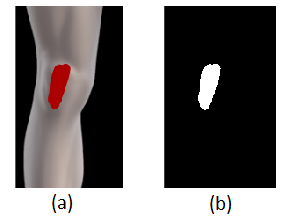
\includegraphics[width=0.4\textwidth]{figures/cropbin7}
\caption{Image consisting of a binary matrix where white color represents the pain pixels.}
\label{fig:cropbin7}
\end{figure}

\subsection{Regions}
The second representation of the data is a matrix consisting of vectors with 20 values which indicate pain in relation to knee regions. 
The knee regions shown in figure \ref{fig:atlas} are converted into a matrix consisting of 20 values, which represent each knee regions. This matrix is superimposed to the binary image of the pain map, which results in a matrix with pain represented in each knee region. In figure \ref{fig:binregions} is there two illustrations of regions with different values (figure \ref{fig:binregions}(a)) and the pain in the specific regions (figure \ref{fig:binregions}(b)).

\begin{figure} [H]
\centering
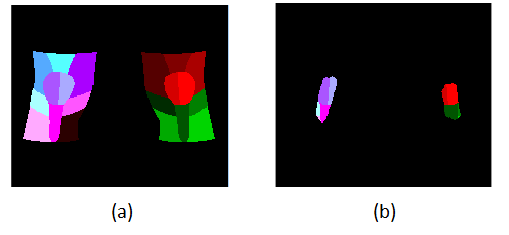
\includegraphics[width=0.8\textwidth]{figures/binregions}
\caption{(a) Knee regions and (b) pain in the specific regions.}
\label{fig:binregions}
\end{figure}

\noindent
After superimposing the two matrices, knee regions and pain, the number of pixels in each active knee region is found. This number is compared to the total number of pixels that are in each knee region, so knee regions with less than 15 \% pain are excluded. WHY 15\%. As an result is a vector with 20 values created.


\subsection{Superimposed morphology and regions}
The third representation of the data is a matrix consisting of subject's pain divided into the knee regions.
\noindent
In this representation the superimposed matrix from the second data representation is used. Since the data representation should reflect the morphology of the pain and divide the pain into the different knee regions is one-hot encoding used. One-hot encoding is a way to separate categorical data into binary data \citep{Harris2012}. This means that the 20 values for each knee region do not have a correlation. After one-hot encoding the superimposed matrix consists of 20 layers where each layer represents a knee region.



%-----------------------results ---------------------------
%\chapter{Results}



\begingroup
\raggedright

\bibliographystyle{unsrtnat}
\bibliography{bib}
%\urlstyle{same}
%
%
%\printbibliography
%\cleardoublepage

\endgroup

%-----------------------Appendix-------------------------
\appendix

\chapter{\large Knee injury and Ostearthritis Outcome Score (KOOS) \citep{KOOS2016}}\label{app:KOOS}
\begin{figure} [H]
\centering
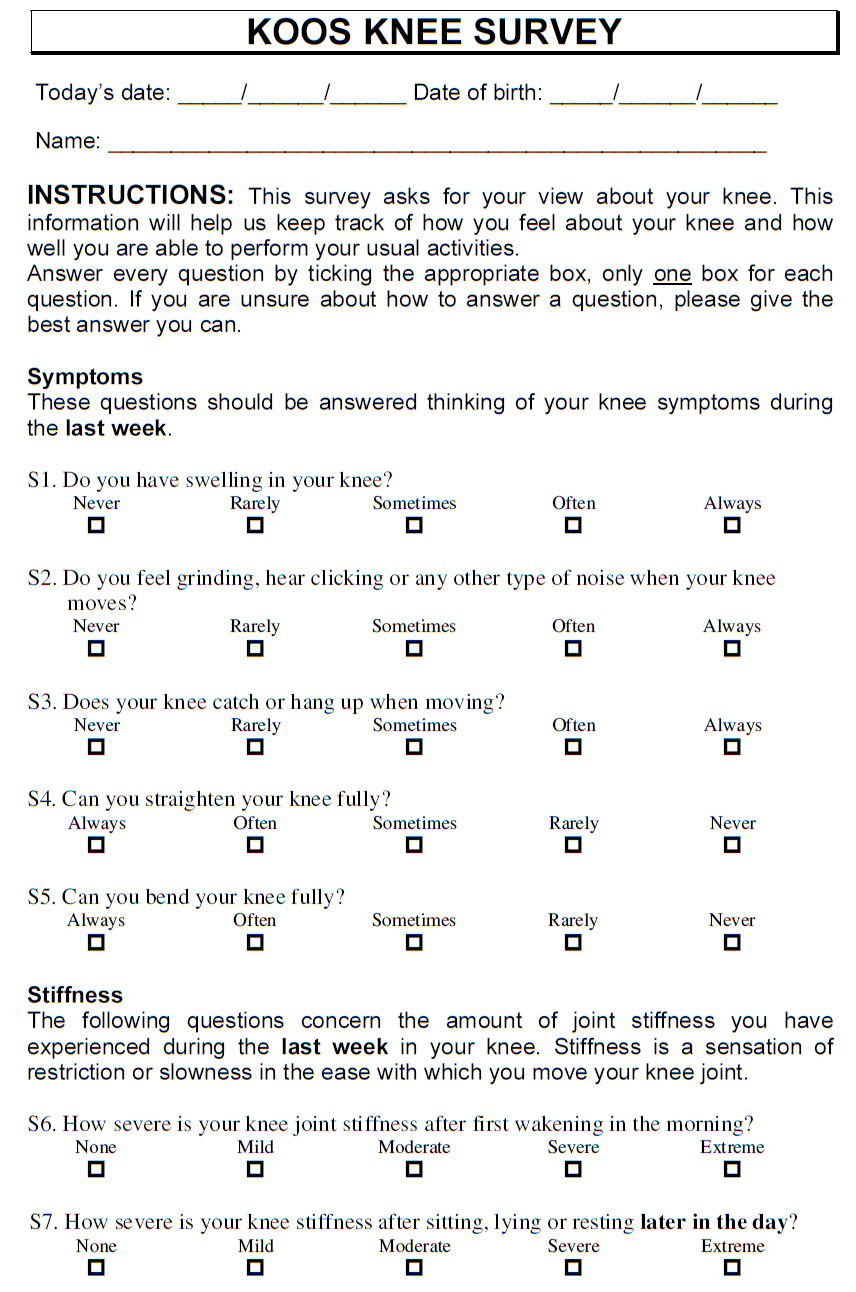
\includegraphics[width=0.85\textwidth]{figures/KOOS1}
\end{figure}

\begin{figure} [H]
\centering
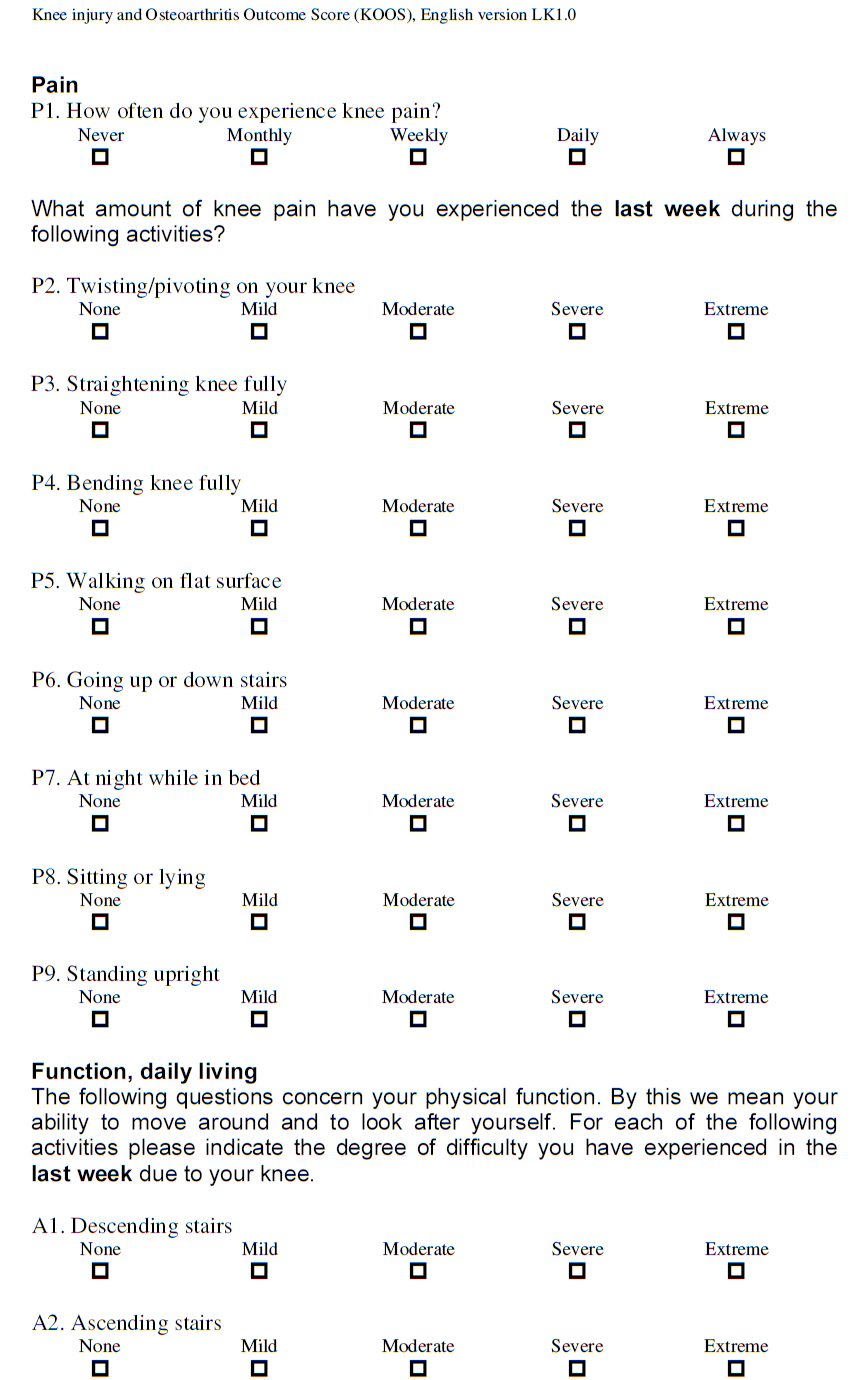
\includegraphics[width=0.95\textwidth]{figures/KOOS2}
\end{figure}


\begin{figure} [H]
\centering
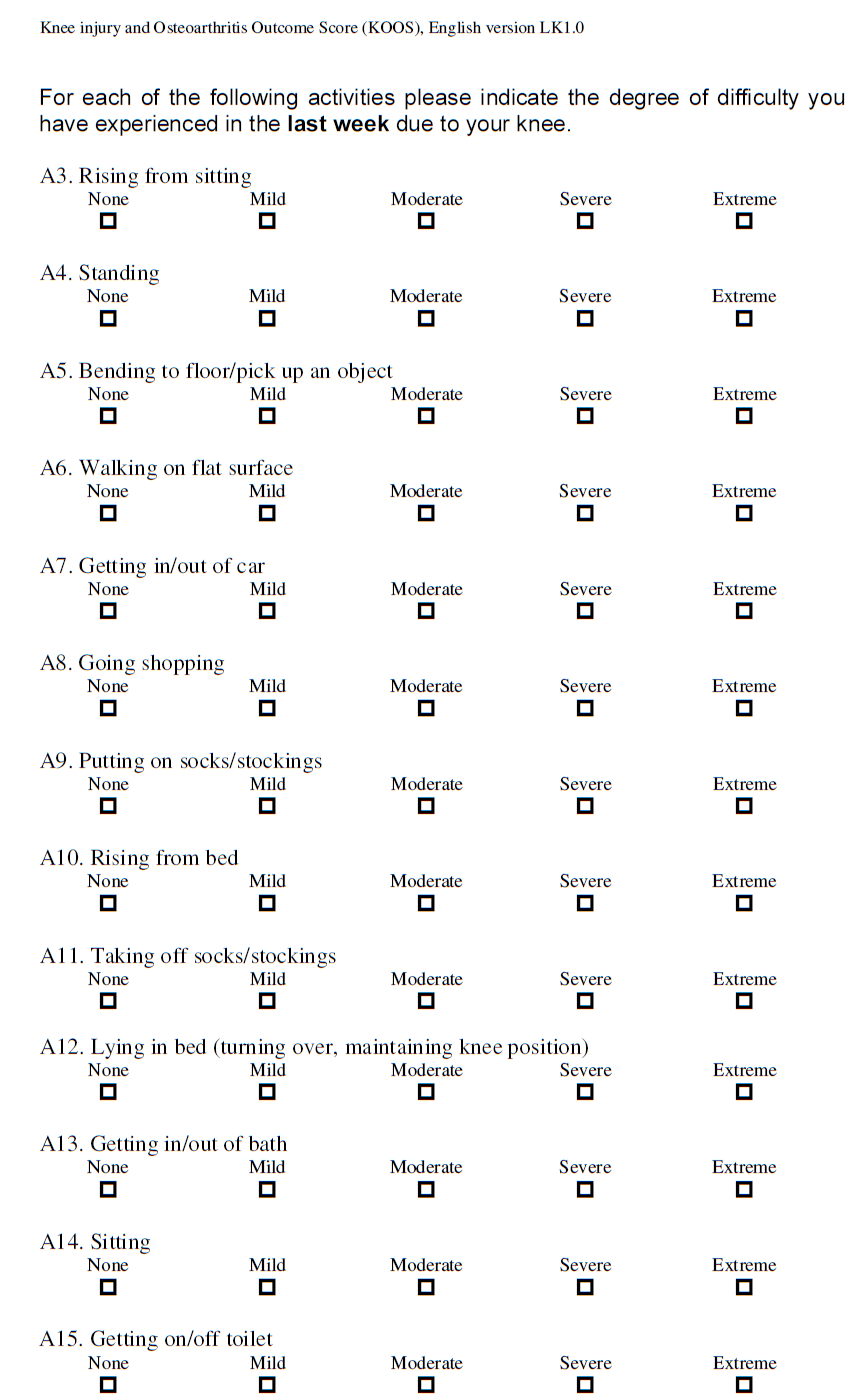
\includegraphics[width=0.9\textwidth]{figures/KOOS3}
\end{figure}


\begin{figure} [H]
\centering
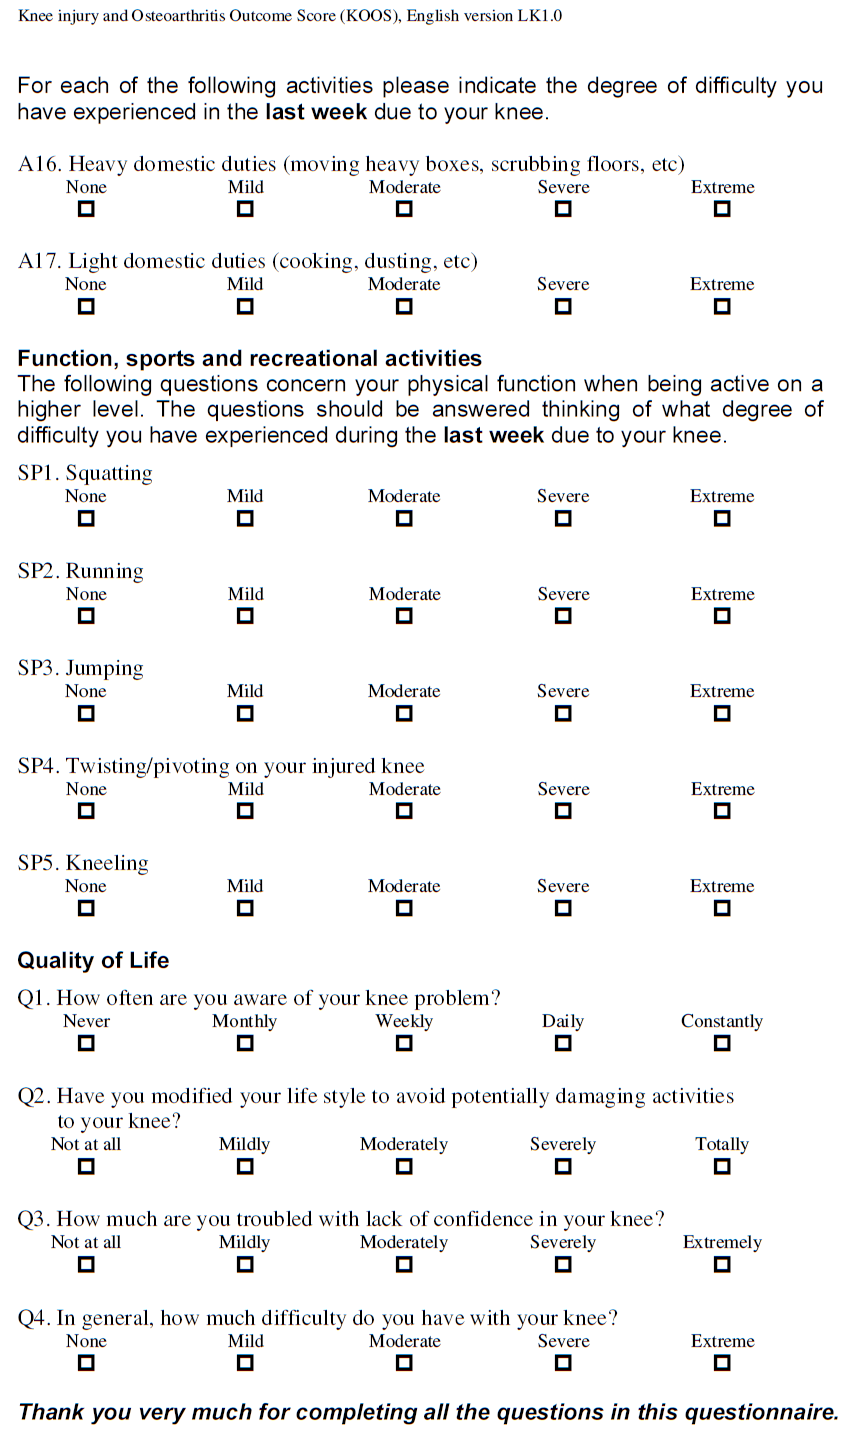
\includegraphics[width=0.95\textwidth]{figures/KOOS4}
\end{figure}


\chapter{\large Threshold analysis}\label{app:thresholds}
\begin{figure} [H]
\centering
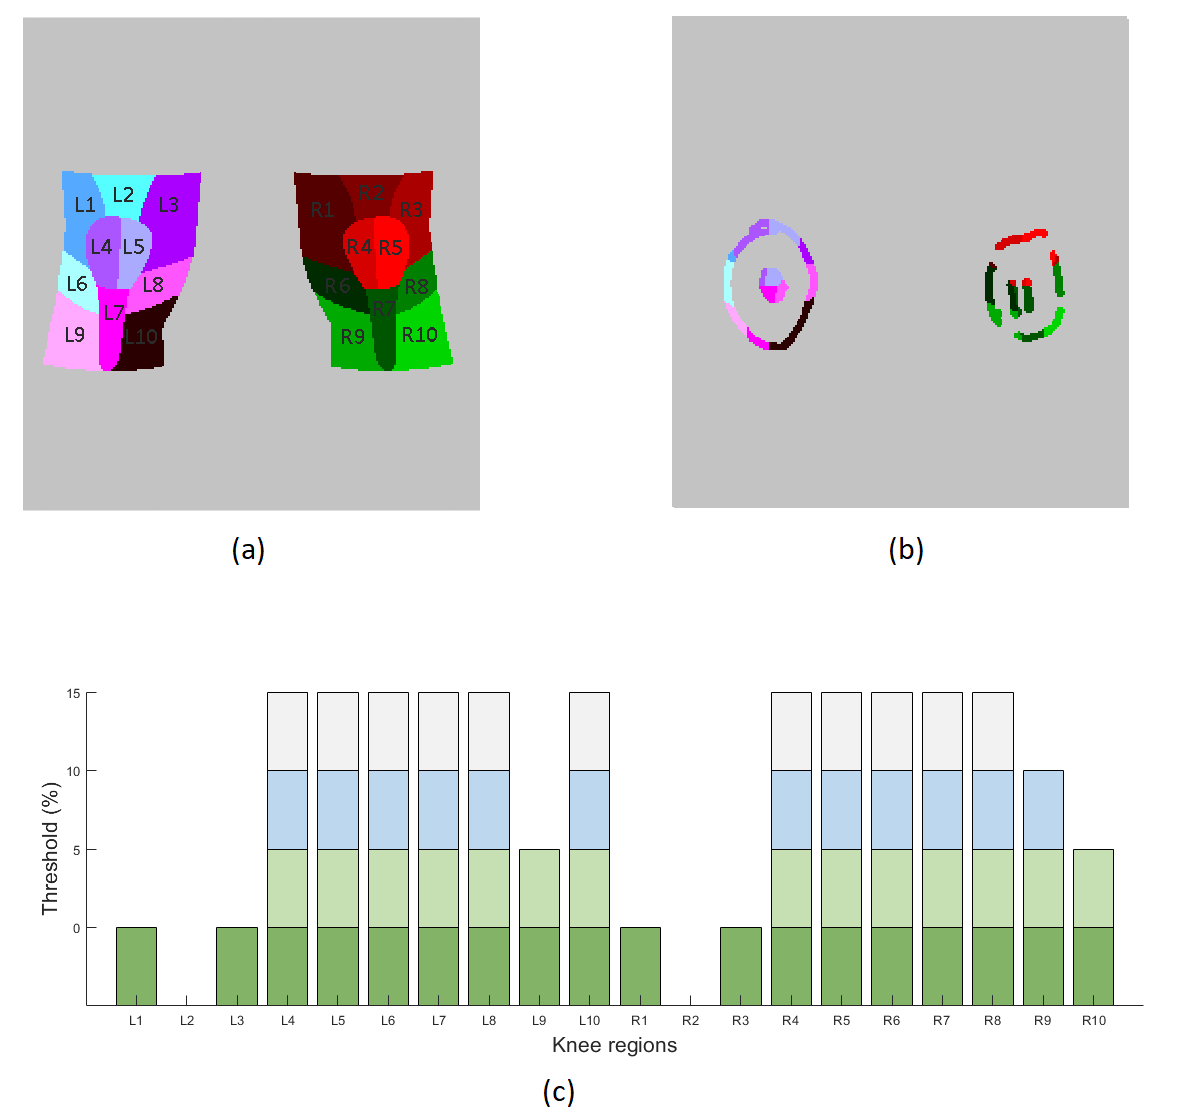
\includegraphics[width=1\textwidth]{figures/threshold52}
\end{figure}

\begin{figure} [H]
\centering
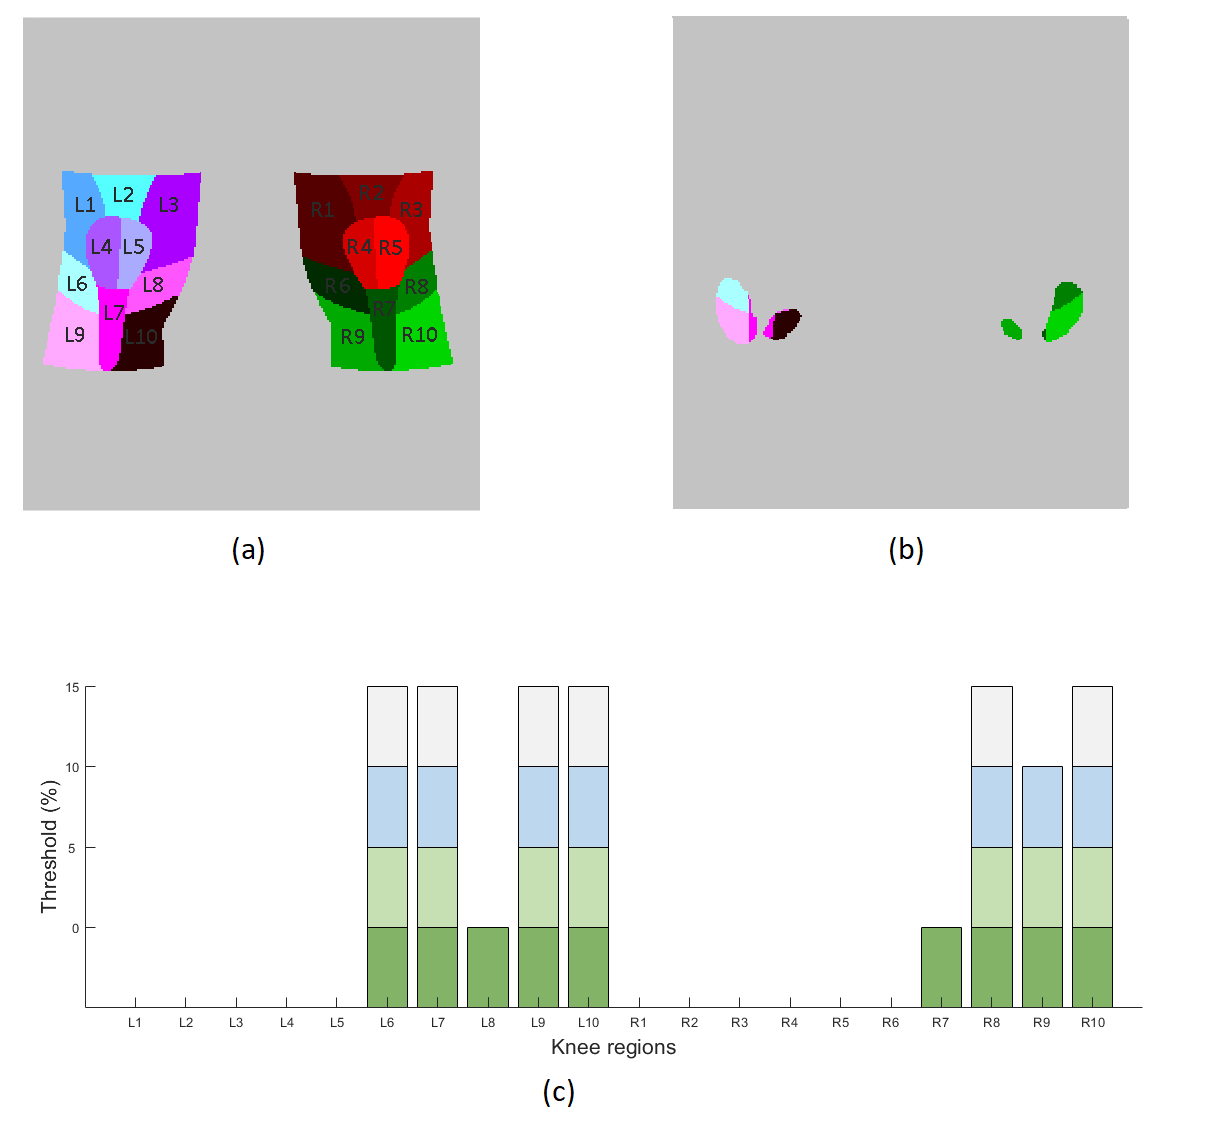
\includegraphics[width=1\textwidth]{figures/threshold67}
\end{figure}

\begin{figure} [H]
\centering
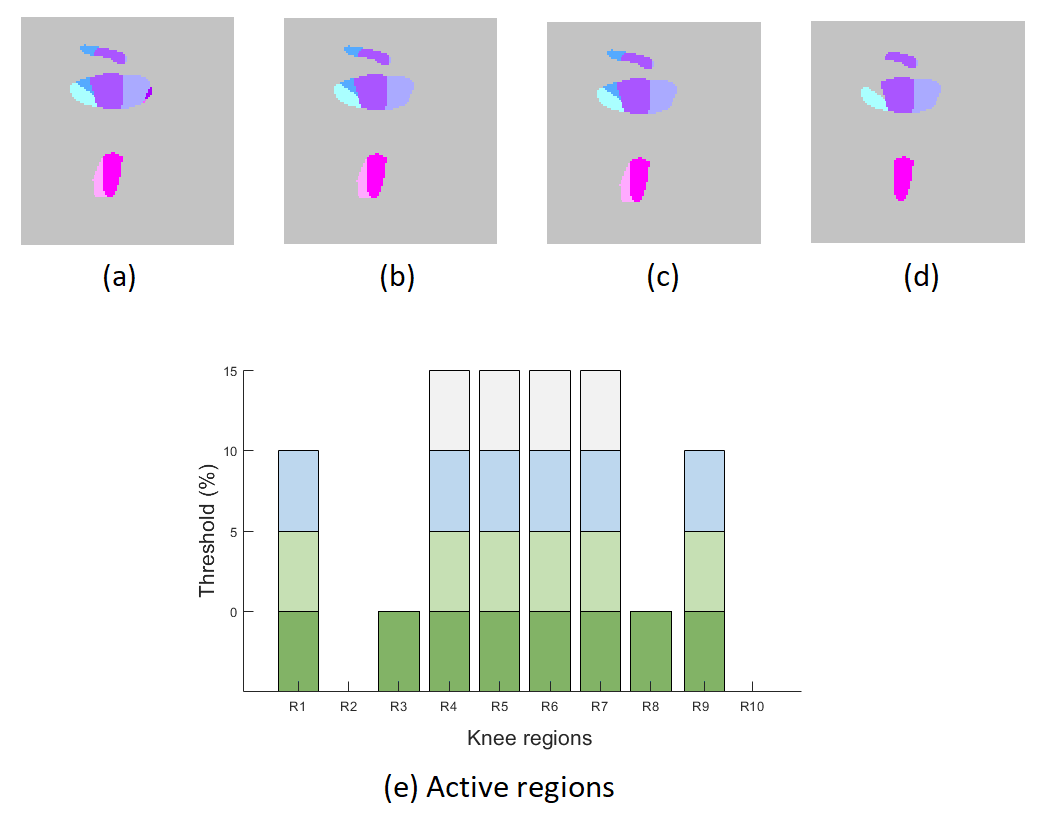
\includegraphics[width=1\textwidth]{figures/threshold125}
\end{figure}

\begin{figure} [H]
\centering
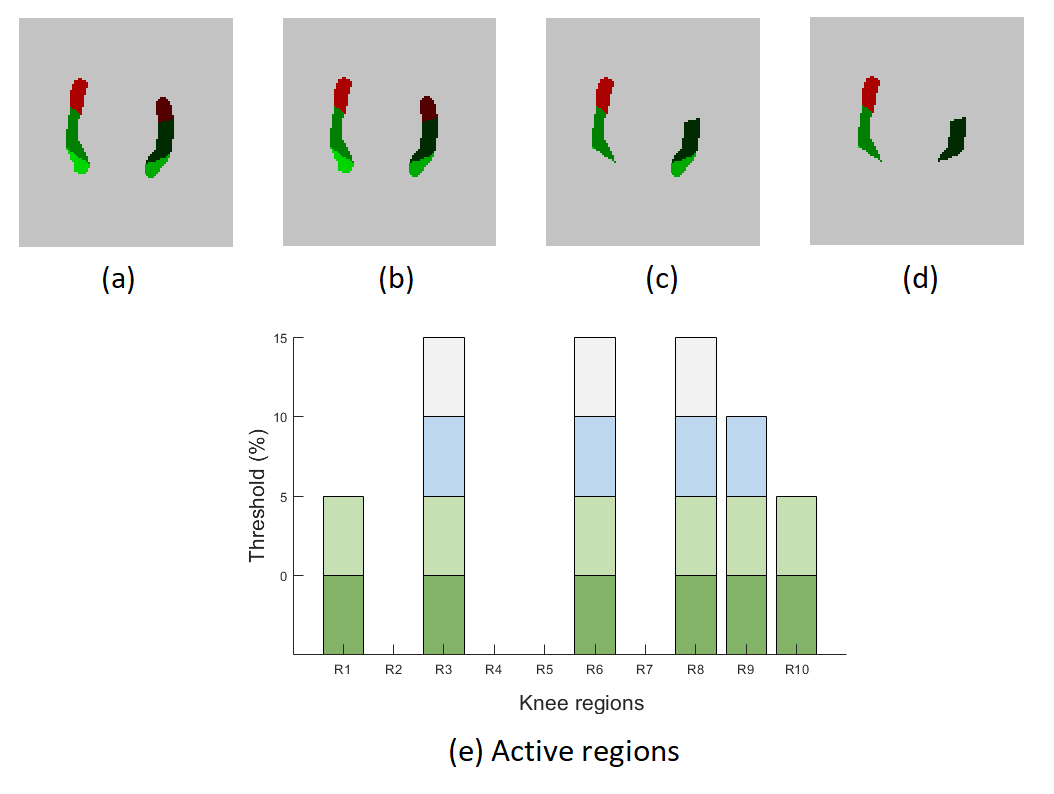
\includegraphics[width=1\textwidth]{figures/threshold206}
\end{figure}

\chapter{\large Architecture of the deep learning models}\label{app:model}
\begin{figure} [H]
\centering
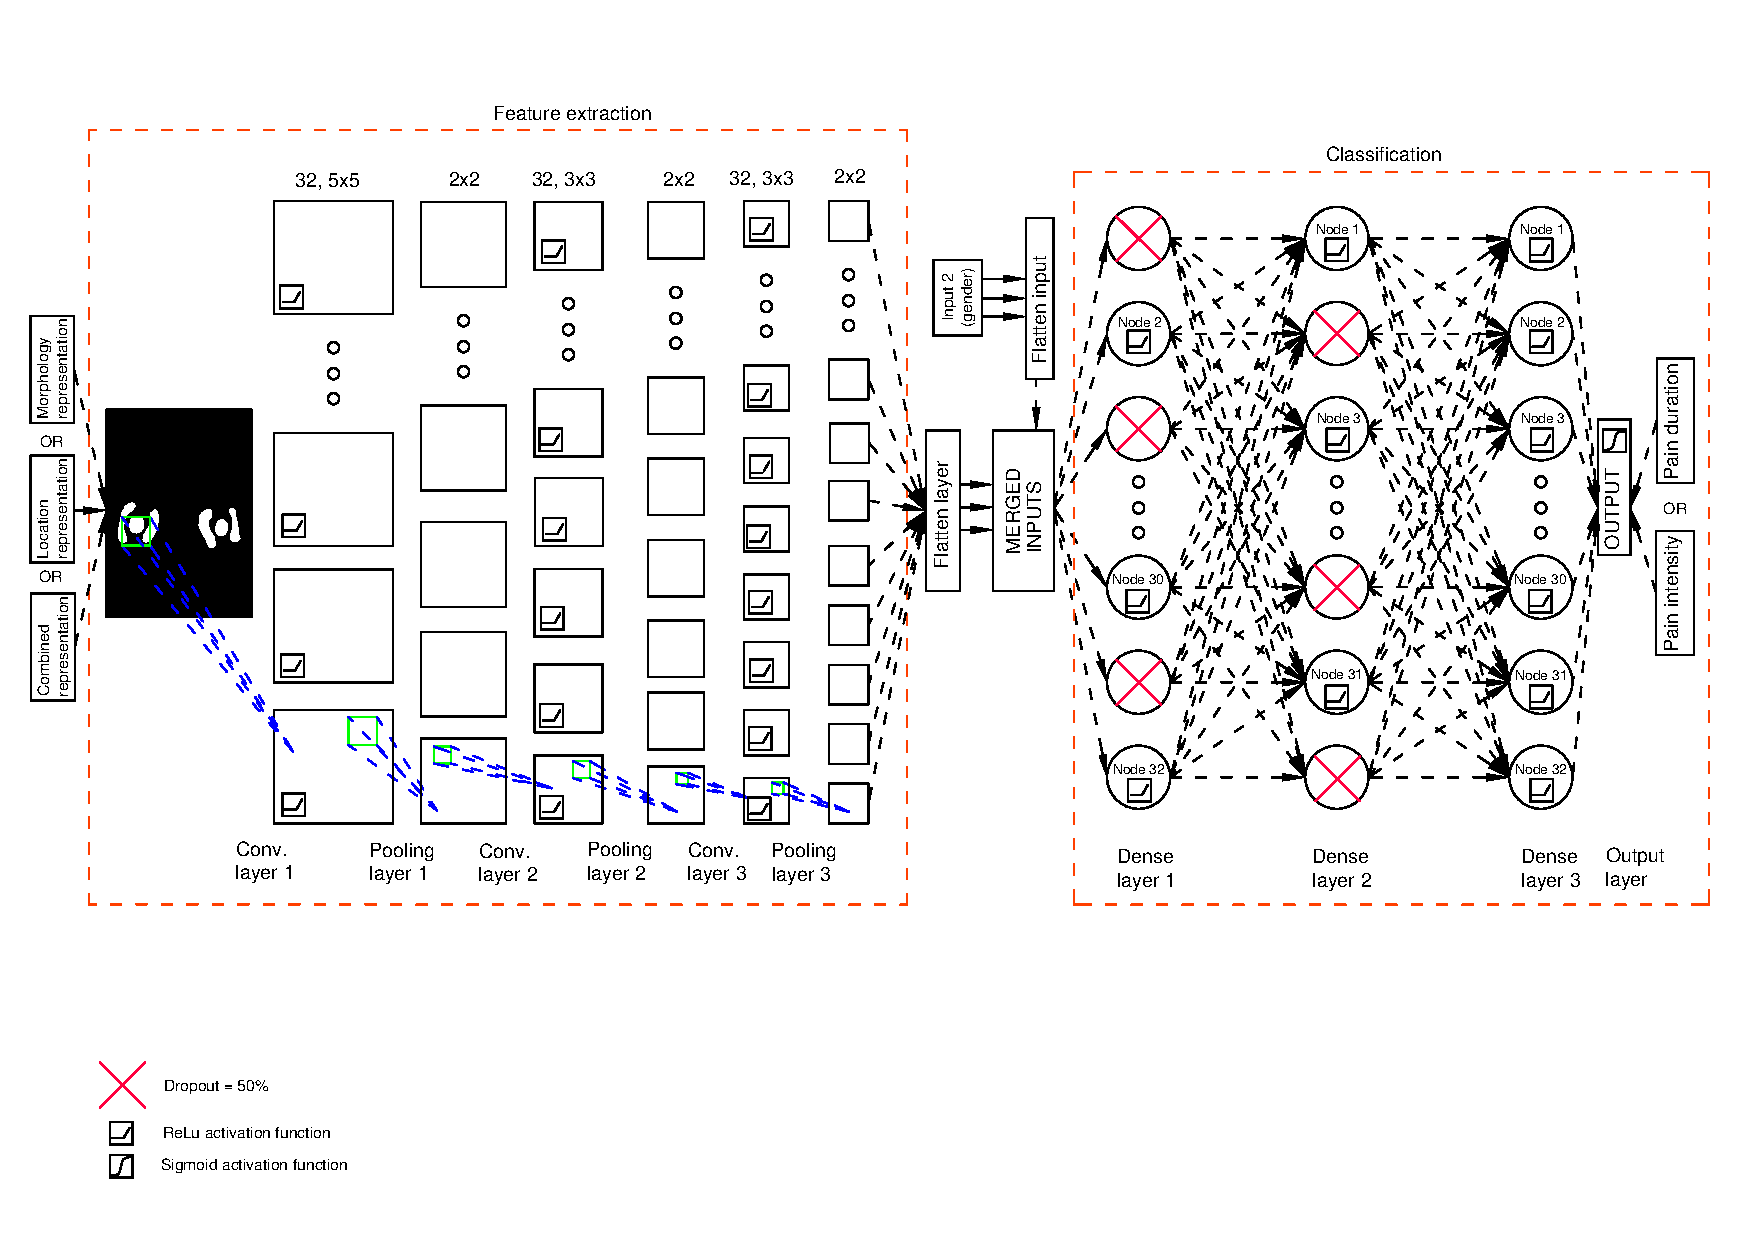
\includegraphics[angle=270, width=1\textwidth]{figures/appModels1.pdf}
\end{figure}

\chapter{\large Optimization parameters} \label{app:opti}
\documentclass[12pt,a4paper]{article}
\usepackage[latin1]{inputenc}
\usepackage[english]{babel}
\usepackage{amsmath}
\usepackage{amsfonts}
\usepackage{amssymb}
\usepackage{makeidx}
\usepackage{graphicx}
\usepackage{booktabs}

\usepackage{caption}
\usepackage{float}
\usepackage{lmodern}
\usepackage[left=2cm,right=2cm,top=2cm,bottom=2cm]{geometry}
\author{Mads Krsitensen}
\begin{document}


\begin{table}[]
\centering
\begin{tabular}{ccccccc}
\hline
\multicolumn{7}{c}{\textbf{Location-representation}}                                                                                                                                                                                                                                                                     \\ \hline
\multicolumn{1}{l}{}                              & \multicolumn{3}{c}{Pain duration}                                                                                                 & \multicolumn{3}{c}{Pain intensity}                                                                                               \\ \cline{2-7} 
\multicolumn{1}{l}{}                              & \begin{tabular}[c]{@{}c@{}}Avg. \\ Accuracy\end{tabular} & $\pm$ SD & \begin{tabular}[c]{@{}c@{}}Chosen \\ parameter\end{tabular} & \begin{tabular}[c]{@{}c@{}}Avg \\ Accuracy\end{tabular} & $\pm$ SD & \begin{tabular}[c]{@{}c@{}}Chosen \\ parameter\end{tabular} \\ \cline{2-7} 
\multicolumn{1}{l}{\textbf{Learning rate:}}       &                                                          &          &                                                             &                                                         &          &                                                             \\
0.1                                               & 56.08                                                    & 13.35    &                                                             & 63.92                                                   & 12.37    &                                                             \\
0.01                                              & 56.08                                                    & 13.35    & X                                                           & 63.92                                                   & 12.37    & X                                                           \\
0.001                                             & 56.08                                                    & 13.35    &                                                             & 63.92                                                   & 12.37    &                                                             \\ \hline
\multicolumn{1}{l}{\textbf{Kernal inintializer:}} &                                                          &          &                                                             &                                                         &          &                                                             \\
normal                                            & 56.08                                                    & 13.35    &                                                             & 63.92                                                   & 12.37    &                                                             \\
glorot\_normal                                    & 56.08                                                    & 13.35    &                                                             & 63.92                                                   & 12.37    &                                                             \\
glorot\_uniform                                   & 56.08                                                    & 13.35    & X                                                           & 63.92                                                   & 12.37    & X                                                           \\ \hline
\multicolumn{1}{l}{\textbf{Neurons:}}             &                                                          &          &                                                             &                                                         &          &                                                             \\
8                                                 & 56.08                                                    & 13.35    &                                                             & 63.92                                                   & 12.37    &                                                             \\
16                                                & 56.08                                                    & 13.35    & X                                                           & 63.92                                                   & 12.37    & X                                                           \\
32                                                & 56.08                                                    & 13.35    &                                                             & 63.92                                                   & 12.37    &                                                             \\ \hline
\multicolumn{1}{l}{\textbf{Epochs, Batch size:}}  &                                                          &          &                                                             &                                                         &          &                                                             \\
100, 10                                           & 56.08                                                    & 13.35    &                                                             & 63.92                                                   & 12.37    &                                                             \\
100, 20                                           & 56.08                                                    & 13.35    &                                                             & 63.92                                                   & 12.37    &                                                             \\
100, 30                                           & 56.08                                                    & 13.35    &                                                             & 63.92                                                   & 12.37    &                                                             \\
120, 10                                           & 56.08                                                    & 13.35    &                                                             & 63.92                                                   & 12.37    &                                                             \\
120, 20                                           & 56.08                                                    & 13.35    & X                                                           & 63.92                                                   & 12.37    & X                                                           \\
120, 30                                           & 56.08                                                    & 13.35    &                                                             & 63.92                                                   & 12.37    &                                                             \\
140, 10                                           & 52.12                                                    & 11.02    &                                                             & 63.92                                                   & 12.37    &                                                             \\
140, 20                                           & 56.08                                                    & 13.35    &                                                             & 63.92                                                   & 12.37    &                                                             \\
140, 30                                           & 56.08                                                    & 13.35    &                                                             & 63.92                                                   & 12.37    &                                                             \\ \hline
\end{tabular}
\caption{Results from the grid search for the LR}
\label{tab:GridLoc}
\end{table}



\begin{table}[]
\centering

\begin{tabular}{ccccccc}
\hline
\multicolumn{7}{c}{\textbf{Location-representation}}                                                                                                                                                                                                                                                                     \\ \hline
\multicolumn{1}{l}{}                              & \multicolumn{3}{c}{Pain duration}                                                                                                 & \multicolumn{3}{c}{Pain intensity}                                                                                               \\ \cline{2-7} 
\multicolumn{1}{l}{}                              & \begin{tabular}[c]{@{}c@{}}Avg. \\ Accuracy\end{tabular} & $\pm$ SD & \begin{tabular}[c]{@{}c@{}}Chosen \\ parameter\end{tabular} & \begin{tabular}[c]{@{}c@{}}Avg \\ Accuracy\end{tabular} & $\pm$ SD & \begin{tabular}[c]{@{}c@{}}Chosen \\ parameter\end{tabular} \\ \cline{2-7} 
\multicolumn{1}{l}{\textbf{Learning rate:}}   &   &   &   &   &   &     \\
0.1        		& 58.50     & 10.50   &        & 68.07    & 9.27    & X     \\
0.01       		& 60.50     & 7.22   & X       & 60.24    & 10.10   &      \\
0.001      		& 56.00     & 8.00   &         & 64.46    & 9.20    &       \\ \hline
\multicolumn{1}{l}{\textbf{Kernal inintializer:}} &  &  &  &  &  &       \\
normal      	& 45.00     & 7.75   &        & 62.65     & 9.74    &       \\
glorot\_normal 	& 48.50 	& 9.50   &        & 62.65     & 9.74    &  X     \\
glorot\_uniform & 58.50 	& 5.50   & X      & 62.04     & 7.97    &      \\ \hline
\multicolumn{1}{l}{\textbf{Neurons:}} &  &  &  &  &  &  \\
16        		& 54.50    	& 13.87   &        & 64.46     & 8.61    & X     \\
32              & 60.50     & 8.20    & X      & 62.05     & 8.89    &       \\
64              & 60.50     & 2.69    &        & 60.24     & 9.29    &       \\ \hline
\multicolumn{1}{l}{\textbf{Epochs, Batch size:}}  &  &  &  &  &  &   \\
100, 10         & XX     & XX   &        & 64.46     & 8.19    &       \\
100, 20         & XX     & XX   &        & 62.65     & 9.74    &       \\
100, 30         & XX     & XX   &        & 62.65     & 9.74    &       \\
120, 10         & XX     & XX   &        & 65.06     & 8.81    &       \\
120, 20         & XX     & XX   &        & 62.65     & 9.74    &       \\
120, 30         & XX     & XX   &        & 62.65     & 9.74    &       \\
140, 10         & XX     & XX   &        & 69.88     & 9.49    & X     \\
140, 20         & XX     & XX   &        & 59.64     & 9.54    &       \\
140, 30         & XX     & XX   &        & 62.65     & 9.74    &       \\ \hline
\end{tabular}
\caption{Results from the grid search for the MR}
\label{tab:GridMorph}
\end{table}




\begin{table}[]
\centering
\begin{tabular}{ccccccc}
\hline
\multicolumn{7}{c}{\textbf{Location-representation}}                                                                                                                                                                                                                                                                     \\ \hline
\multicolumn{1}{l}{}                              & \multicolumn{3}{c}{Pain duration}                                                                                                 & \multicolumn{3}{c}{Pain intensity}                                                                                               \\ \cline{2-7} 
\multicolumn{1}{l}{}                              & \begin{tabular}[c]{@{}c@{}}Avg. \\ Accuracy\end{tabular} & $\pm$ SD & \begin{tabular}[c]{@{}c@{}}Chosen \\ parameter\end{tabular} & \begin{tabular}[c]{@{}c@{}}Avg \\ Accuracy\end{tabular} & $\pm$ SD & \begin{tabular}[c]{@{}c@{}}Chosen \\ parameter\end{tabular} \\ \cline{2-7} 
\multicolumn{1}{l}{\textbf{Learning rate:}}   &   &   &   &   &   &     \\
0.1        		& 66.16     & 8.52   & X       & 60.98    & 14.67    &       \\
0.01       		& 52.02     & 9.79   &         & 60.98    & 15.13    &      \\
0.001      		& 54.04     & 10.67  &         & 62.80    & 14.35    & X      \\ \hline
\multicolumn{1}{l}{\textbf{Kernal inintializer:}} &  &  &  &  &  &       \\
normal      	& 62.63     & 8.45   &        & 61.59     & 15.35    &       \\
glorot\_normal 	& 63.63 	& 6.45   &        & 61.59     & 15.35    &       \\
glorot\_uniform & 70.20 	& 8.49   & X      & 61.59     & 15.35    & X     \\ \hline
\multicolumn{1}{l}{\textbf{Neurons:}} &  &  &  &  &  &  \\
8        		& 67.17    	& 6.49    & X      & 61.59     & 15.35    & X     \\
16              & 60.10     & 10.03   &        & 61.59     & 15.35    &       \\
32              & 62.12     & 10.92   &        & 61.59     & 15.35    &       \\ \hline
\multicolumn{1}{l}{\textbf{Epochs, Batch size:}}  &  &  &  &  &  &   \\
100, 10         & 61.11     & 4.85   &        & 61.59     & 15.35    &       \\
100, 20         & 58.08     & 8.81   &        & 61.59     & 15.35    &       \\
100, 30         & 61.61     & 4.32   &        & 61.59     & 15.35    &       \\
120, 10         & 63.13     & 5.48   &        & 61.59     & 15.35    &       \\
120, 20         & 62.12     & 10.57  &        & 61.59     & 15.35    & X     \\
120, 30         & 68.68     & 6.90   & X      & 61.59     & 15.35    &       \\
140, 10         & 60.61     & 10.30  &        & 61.59     & 15.35    &       \\
140, 20         & 64.65     & 8.75   &        & 61.59     & 15.35    &       \\
140, 30         & 64.65     & 8.34   &        & 61.59     & 15.35    &       \\ \hline
\end{tabular}
\caption{Results from the grid search for the CR}
\label{tab:GridCombined}
\end{table}

\end{document}


%\fi
\end{document}